\documentclass[a4paper, 12pt, oneside]{report} % Fixed 13pt issue

\bibliography{Bibliography} % Include the bibliography file
\usepackage{lmodern} % Provides bold small caps font
\linespread{1.5} % Line spacing
\pagestyle{plain}
\usepackage{geometry} % Page margins
\geometry{a4paper, top=3cm, bottom=3cm, left=3cm, right=3cm, bindingoffset=5mm}

\usepackage{graphicx}
\graphicspath{{images/}{./}} % Ensure images are found

\usepackage{multicol} % Multiple columns
\usepackage{amsmath}
\usepackage{ragged2e} % Text alignment
\usepackage{minitoc} % Mini-tables of contents
\usepackage[english]{babel} % Main language
\usepackage{csquotes} % Fixes 'babel/polyglossia' warning
\usepackage{ragged2e}
\usepackage{subcaption}
\usepackage{float}
\usepackage{tikz}
\usetikzlibrary{shapes.geometric, arrows.meta, positioning}
\tikzstyle{process} = [rectangle, rounded corners=5pt, minimum width=3.5cm, minimum height=1cm, text centered, draw=blue!50!black, fill=blue!20]
\tikzstyle{arrow} = [thick, ->, >=stealth]

\usepackage{booktabs}



\nomtcrule 
\addto{\captionsenglish}{% Making babel aware of special titles
  \renewcommand{\mtctitle}{Summary}
}

\usepackage[backend=biber,style=numeric,sorting=none]{biblatex}  
\addbibresource{Bibliography.bib}  % Ensure this matches your .bib filename


\usepackage{comment}
\usepackage{xpatch}
\usepackage{blindtext}

% Modify chapter headings to be centered
\makeatletter
\xpatchcmd{\@makeschapterhead}{%
  \Huge \bfseries  #1\par\nobreak%
}{%
  \Huge \bfseries\centering #1\par\nobreak%
}{\typeout{Patched makeschapterhead}}{\typeout{Patching of @makeschapterhead failed}}

\xpatchcmd{\@makechapterhead}{%
  \huge\bfseries \@chapapp\space \thechapter
}{%
  \huge\bfseries\centering \@chapapp\space \thechapter
}{\typeout{Patched @makechapterhead}}{\typeout{Patching of @makechapterhead failed}}
\makeatother

\usepackage{fancyhdr}
\usepackage[export]{adjustbox}
\usepackage{hyperref} % Hyperlinks
\hypersetup{
    colorlinks=true,
    citecolor=cyan,
    linkcolor=black,
    urlcolor=black,
    pdftitle= Analysis of Indicators to Assess the Resilience of Transport Networks in an Interregional Context,
    pdfauthor=Seyedreza Aghayarikordkandi,
}

\usepackage{booktabs} % Tables
\usepackage{multirow}
\usepackage[table,xcdraw]{xcolor}
\usepackage{lscape}
\usepackage{float}
\usepackage{wrapfig}
\usepackage{tikz}
\usetikzlibrary{shapes.geometric, arrows, positioning}

\hypersetup{
    colorlinks=true,        % Disable colored links
    linkcolor=black,        % Color of internal links (sections, etc.)
    citecolor=black,        % Color of citations
    filecolor=black,        % Color of file links
    urlcolor=black          % Color of external links
}

\setcounter{secnumdepth}{4}
% Document begins here
\begin{document}

% Title Page
\begin{titlepage}
\begin{center}
    {\scshape\LARGE UNIVERSIT\`A DEGLI STUDI DI NAPOLI \ FEDERICO II \par}
    \vspace{1cm}
    
\includegraphics[width=0.3\textwidth]{images/logo.jpg} \par
    \vspace{0.7cm}
    {\scshape\Large FACULTY OF ENGINEERING \par}
    \vspace{0.5cm}
    {\scshape\normalsize Master’s Degree in Transportation Engineering and Mobility \par}
    \vspace{0.3cm}
    {\scshape\small DEPARTMENT OF CIVIL, BUILDING AND ENVIRONMENTAL ENGINEERING \par}
    \vspace{0.3cm}
    
    {\scshape\normalsize\bfseries Analysis of Indicators to Assess the Resilience of Transport Networks in an Interregional Context \par}
    \vspace{0.5cm}
\end{center}

 \begin{minipage}{0.45\textwidth}
    \raggedright
    {\scshape\normalsize \textbf{Supervisor:}} \\
    Prof. Luigi Pariota \\
    {\scshape\normalsize \textbf{Co-supervisor:}} \\
    Dr. Luca Di Costanzo
    \end{minipage}%
    \begin{minipage}{0.45\textwidth}
    \raggedright
    {\scshape\normalsize \textbf{Candidate:}} \\
    Seyedreza Aghayarikordkandi \\
    \end{minipage}

\vfill

% Bottom of the page
\begin{center}
    {\scshape\large ACADEMIC YEAR 2024/2025}
\end{center}

\end{titlepage}

\begin{abstract}
    \noindent The resilience of transport networks under seismic disturbances is a critical concern for ensuring regional connectivity, accessibility, and post-disaster recovery. This study analyzes the resilience of the Southern Italy transport network under multiple seismic fault scenarios, focusing on network centrality, connectivity indicators, and redundancy analysis to assess the impact of disruptions.

    The methodology integrates network analysis and seismic hazard modeling to evaluate the vulnerability of critical links and nodes. Key indicators such as betweenness centrality, clustering coefficient, average degree, beta index, and gamma index provide insights into the pre- and post-disruption behavior of the network. Redundancy analysis further examines the extent to which travel time increases and zones become disconnected under varying seismic intensities. The study identifies the A16 motorway as a critical corridor, where disruptions significantly affect east-west connectivity, particularly impacting OD pairs between Campania and Puglia. Additionally, the findings highlight that high-intensity seismic events lead to severe network fragmentation, particularly in Benevento, Avellino, and Calabria, due to lower node density and limited alternative routes.

    The results underscore the need for strategic resilience planning, including reinforcing major highways, developing alternative expressways, and implementing emergency rerouting strategies for OD pairs with low redundancy values. The study provides a comprehensive framework for evaluating transport network resilience, offering valuable insights for policymakers and urban planners to mitigate seismic risks and enhance regional connectivity in future disruptions.
\end{abstract}

\newpage 
\dominitoc
\tableofcontents

\addcontentsline{toc}{chapter}{List of Figures}
\listoffigures

\addcontentsline{toc}{chapter}{List of Tables}
\listoftables

\chapter{Introduction}

\section{Background and Motivation}
Transportation systems form the backbone of modern society, facilitating the movement of people, goods, and services while fostering economic growth and social well-being. However, these systems are increasingly vulnerable to natural disasters, climate change, and anthropogenic disruptions, which significantly impact infrastructure reliability, mobility, and network resilience \cite{pescaroli2016}. Disruptions such as earthquakes, landslides, flooding, and infrastructure failures can lead to severe network disruptions, affecting millions of commuters, businesses, and emergency services \cite{gu2020, wu2021}.

Recent disasters highlight the urgency of transport network resilience:
\begin{itemize}
    \item The 2008 Wenchuan earthquake in China triggered over 15,000 landslides, destroying highways and isolating entire regions \cite{tang2011}.
    \item The 2018 Morandi Bridge collapse in Genoa, Italy, killed 43 people, left 600 homeless, and caused an economic disaster, disrupting urban mobility for years \cite{scozzese2019}.
    \item The 2011 Tōhoku earthquake and tsunami in Japan severely damaged rail and road networks, demonstrating the cascading impacts of seismic hazards on transportation systems \cite{krausmann2013}.
\end{itemize}

\hyphenpenalty=1000
\tolerance=1000
\justify Given these challenges, resilience assessment of transportation networks has emerged as a crucial field of study. Resilient networks can withstand, absorb, and recover from shocks, ensuring continued connectivity between key locations before, during, and after disruptions \cite{yang2022}. This thesis develops a resilience assessment framework integrating graph-based network analysis, GIS spatial analysis, and transport simulation using PTV Visum.

\section{Importance of Transport Resilience in Disaster Management}
Critical infrastructure resilience is a key component of disaster management, influencing response times, recovery rates, and economic stability . Among all infrastructures, transportation systems are particularly vulnerable due to their interconnected nature and dependency on structural integrity \cite{gu2020}.

A disruption in one transport link—such as a collapsed bridge or damaged highway—can trigger network-wide consequences, affecting:
\begin{itemize}
    \item Emergency response (delays in medical and rescue services).
    \item Economic stability (increased cost of goods and logistics disruptions).
    \item Public mobility (restricted access to essential services, workplaces, and homes).
\end{itemize}
For example, during Hurricane Katrina (2005) and Hurricane Sandy (2012) in the US, widespread flooding and road failures hindered relief efforts, demonstrating the importance of transport network adaptability in extreme weather events \cite{padgett2008}. Similarly, the Cumbria floods (2009) in the UK caused £34 million in road restoration costs due to bridge collapses \cite{cumbria2010}.

Thus, it is essential to assess and enhance the resilience of transport networks, particularly in seismically active regions like Southern Italy, where seismic faults intersect major transportation corridors.

\section{Research Gap and Challenges}
Current research on transport resilience primarily focuses on either:
\begin{enumerate}
    \item Topological resilience – Evaluating network connectivity and redundancy through graph theory indicators \cite{wang2019}.
    \item Functional resilience – Assessing real-time network performance, including travel time variations, congestion, and rerouting behavior \cite{bell1999}.
\end{enumerate}
However, studying these perspectives separately leads to incomplete resilience assessments. Traditional transport models often fail to integrate:
\begin{itemize}
    \item Land-use dependencies – Urban density, economic activity, and road accessibility.
    \item Environmental hazards – Seismic risk zones, flood-prone areas, and terrain complexity.
    \item Infrastructure stress factors – Road fatigue, bridge load capacity, and maintenance constraints.
\end{itemize}
To address these gaps, this thesis introduces a multi-layered resilience framework that integrates:
\begin{itemize}
    \item Graph-theory-based resilience metrics (Beta Index, Gamma Index, Betweenness Centrality, Clustering Coefficient).
    \item GIS-based spatial risk modeling (earthquake-prone zones, flood-prone areas, critical infrastructure mapping).
    \item Seismic scenario simulations using PTV Visum (travel time variations, route disruptions, network redundancy assessment).
    \item "Augmented link" modeling approach – Incorporating land-use dependencies, infrastructure conditions, and traffic demand levels into resilience assessments \cite{postorino2025}.
\end{itemize}

\section{Research Objectives}
This research aims to develop and apply a resilience assessment framework that:
\begin{enumerate}
    \item Evaluates seismic disruption impacts on transport network connectivity and mobility.
    \item Identifies critical transport links using graph-based and GIS-based resilience indicators.
    \item Assesses network redundancy and recovery capacity using the Redundancy Indicator metric.
    \item Integrates land-use interactions into transport resilience models for enhanced disaster response planning.
    \item Simulates post-disaster network performance under low-intensity (10\% link failure) and high-intensity (40\% link failure) seismic scenarios.
\end{enumerate}

\section{Research Questions}
This thesis seeks to answer the following key research questions:
\begin{enumerate}
    \item How do seismic disruptions impact transport network connectivity and redundancy?
    \item Which transport links and nodes are most critical for post-disaster mobility?
    \item How do redundancy metrics (Beta, Gamma, Clustering Coefficient) evolve under disruptions?
    \item How do land-use patterns influence network resilience and recovery strategies?
    \item What resilience strategies can improve transport network adaptability in seismic-prone regions?
\end{enumerate}

\section{Significance of the Study}
This research contributes to transport resilience analysis by:
\begin{itemize}
    \item Bridging the gap between topological and functional resilience.
    \item Integrating land-use dependencies into resilience assessments.
    \item Developing a GIS-based risk analysis framework for seismic disruptions.
    \item Providing a decision-support system for urban planners and policymakers.
\end{itemize}
By combining transport modeling, spatial analysis, and graph-based metrics, this study offers a comprehensive methodology to enhance transport network resilience in disaster-prone areas.



 
\chapter{Literature review}

\section{Introduction}
The resilience of transport networks has become a critical focus in infrastructure planning, particularly in regions prone to disruptions such as natural disasters, extreme weather events, and structural failures. A resilient transport network ensures continued connectivity, minimizes delays, and provides alternative routes when disruptions occur. Resilience in transport networks refers to the system's ability to absorb, adapt to, and recover from disruptions while maintaining essential functions and services \cite{holling1973}. It encompasses network robustness, redundancy, and adaptive capacity, ensuring that transport infrastructure can continue functioning under various stress conditions \cite{taylor2017}.

Closely related to resilience is the concept of redundancy, which refers to the presence of alternative routes or backup infrastructure that can sustain functionality when primary links fail. A network with high redundancy can reallocate traffic through alternative paths, reducing the impact of disruptions and preventing system-wide failures \cite{zhang2018}. Redundancy is particularly important in interregional transport networks, where disruptions to major highways, bridges, or rail lines can have widespread economic and social consequences.

This chapter reviews key studies and methodologies used to evaluate transport network resilience, with a particular focus on graph theory indicators and GIS-based spatial analysis. Graph theory provides a quantitative framework for analyzing network connectivity, redundancy, and structural robustness, while Geographic Information Systems (GIS) facilitate spatial modeling and visualization of disruptions. The combination of these methodologies allows researchers to identify critical links and nodes, assess network redundancy, and propose infrastructure improvements aimed at enhancing resilience.

The literature review is structured into several sections. The first section discusses the role of graph theory indicators in assessing transport network performance, including key metrics such as beta index, gamma index, clustering coefficient, and betweenness centrality. These indicators provide insights into network complexity, connectivity, and the impact of disruptions on overall system functionality. The next section focuses on seismic disruptions and their impact on transport networks, highlighting studies that assess the vulnerability of critical infrastructure components such as roads, bridges, and tunnels in seismically active regions.

Further sections explore the integration of graph theory and GIS methodologies for resilience assessments, examining how these tools have been applied to urban and interregional transport networks. Studies that combine network topology with spatial data have proven effective in predicting disruption impacts and guiding infrastructure resilience strategies. The final section synthesizes findings from previous research and identifies gaps in the existing literature, particularly concerning the assessment of interregional transport networks, which often face unique challenges due to their scale, jurisdictional boundaries, and varied infrastructure conditions.

By reviewing these methodologies and case studies, this chapter establishes a foundation for analyzing transport network resilience using graph-based indicators in an interregional context. The findings from the literature will inform the methodological approach presented in the next chapter, ensuring a comprehensive framework for evaluating and improving transport network resilience across regions.

\section{Graph Theory Applications in Transport Network Resilience}
Graph theory has emerged as a powerful tool in the study of transport network resilience, providing a mathematical framework to analyze network connectivity, structure, and redundancy. By representing transport networks as graphs composed of nodes (intersections, stations) and edges (roads, railways), graph theory enables the evaluation of how networks function under normal conditions and how they respond to disruptions.

Historically, transport network vulnerability assessments have largely relied on accessibility-based approaches, where the impact of disruptions is measured in terms of accessibility loss and travel cost increases. Many studies have evaluated network vulnerability by assessing connectivity reliability, generalized travel cost, and accessibility indicators \cite{taylor2006, jenelius2006}. These methods focus on how disruptions affect the ease of reaching destinations and the efficiency of transport services. However, graph theory provides a complementary and more structured approach, allowing for the quantification of redundancy, network robustness, and interconnectivity, which are essential for understanding resilience.

In this context, \cite{thottolil2021} investigate the topology of Bangalore’s road networks, focusing on connectivity and coverage through graph theory. Their research highlights the relationship between road connectivity and the development of the road transport system, utilizing OpenStreetMap data to compute various topological measures. Through correlation analysis, they demonstrate the strength of the relationship among these indicators and propose a model linking connectivity indices with network density metrics. This model offers valuable insights into how urban transport networks can be optimized for efficiency and resilience.

Graph-based approaches in transport resilience studies have demonstrated their effectiveness in assessing the structural properties of networks, identifying critical links and nodes, and predicting the impact of disruptions on overall connectivity. The ability of graph theory to quantify network robustness allows for a systematic evaluation of different resilience indicators, including connectivity indices, redundancy measures, and centrality metrics. These indicators provide transport planners with the necessary tools to design networks that can withstand disruptions and maintain functional accessibility.

By applying graph theory to transport resilience analysis, researchers have been able to develop models that can be adapted to various urban and interregional contexts. These models assist in the optimization of infrastructure investments, ensuring that road networks remain efficient and reliable under different operational conditions. The ability to integrate graph-theoretic analysis with real-world transport data allows for more informed decision-making, contributing to the development of sustainable and resilient transportation systems.
\section{Seismic Disruptions and Their Impact on Transport Networks}
Seismic disruptions significantly affect the connectivity, redundancy, and resilience of transportation networks in seismically active regions. Earthquakes can cause severe structural damage to transport infrastructure, including roadways, bridges, tunnels, and railway systems, leading to prolonged accessibility disruptions and economic losses. The ability of a transport network to withstand and recover from such disruptions is critical for ensuring mobility, emergency response effectiveness, and overall regional stability.

\cite{dou2023} highlight the critical need for resilience assessments of road transportation infrastructure systems under earthquake impacts, emphasizing the importance of connectivity reliability and travel time evaluations for emergency planning. Their study on the Aba Autonomous Prefecture demonstrates how Monte Carlo simulations can effectively model uncertainties in seismic hazard assessments, revealing vulnerabilities in road assets such as bridges and tunnels. Their findings indicate that the failure of critical transport links during seismic events can lead to network fragmentation, severely affecting evacuation routes and access to essential services.

Seismic risk modeling has increasingly focused on integrating graph-based resilience metrics with geospatial data to assess transport network vulnerabilities. By combining redundancy indicators and structural failure probability models, researchers can identify high-risk zones and propose mitigation strategies to minimize seismic-induced disruptions. Understanding how network connectivity changes due to seismic damage is essential for designing adaptive transport systems that can reroute traffic efficiently when primary corridors become impassable.

The necessity of incorporating connectivity and redundancy metrics into resilience frameworks is underscored by studies such as Dou et al. (2023), which advocate for a data-driven approach to strengthening transport networks in earthquake-prone areas. Their research suggests that proactive infrastructure reinforcement, emergency detour planning, and strategic investment in redundant links can significantly enhance the post-disruption performance of road transportation systems. These findings align with broader efforts to develop seismic resilience strategies that ensure transport networks remain functional even in the aftermath of catastrophic events.

\section{Graph Theory and GIS-Based Resilience Assessment}
Assessing the resilience of transport networks under earthquake-induced disruptions is critical for enhancing community safety and economic stability. Recent studies have highlighted effective methodologies that leverage graph theory and Geographic Information Systems (GIS) to evaluate such resilience. By integrating network topology with spatial data, researchers can assess the vulnerability of transport infrastructure, identify critical network components, and develop targeted mitigation strategies to enhance overall resilience.

\cite{rouhana2020} introduced a novel approach based on graph theory concepts, focusing on the topological properties of the transportation network in Beirut. Their research demonstrated how the road network's configuration influences its resilience against random and targeted failures, revealing that critical network components could be identified to optimize resource allocation and minimize downtime. Their findings emphasize the importance of network redundancy and structural robustness in maintaining connectivity under seismic stress.

In a complementary study \cite{ dapuzzo2022} proposed an innovative methodological framework that integrates geo-statistical approaches to analyze soil properties and predict liquefaction risks. This framework, applied to a district in northern Italy, assessed the economic losses associated with seismic-induced road disruptions, providing a comprehensive evaluation of accessibility impacts during seismic events. The study highlights how integrating geological vulnerability assessments with network topology analysis allows for a more accurate prediction of post-disruption accessibility challenges.

Both studies underscore the importance of utilizing graph-based and GIS-based methodologies to quantify resilience effectively. Graph theory enables researchers to measure network connectivity, redundancy, and vulnerability, while GIS applications provide spatial insights into potential risk factors such as seismic zones, population density, and emergency service accessibility. By combining topological analysis with spatial data, researchers can develop robust planning tools that enhance the resilience of transport networks against earthquake-induced disruptions. These tools contribute to sustainable urban development and disaster preparedness by enabling decision-makers to identify weak points in transport infrastructure and prioritize strategic interventions to strengthen resilience.

\section{Graph-Based Indicators for Transport Network Resilience}
Graph-based indicators play a fundamental role in assessing the resilience of transport networks, particularly in evaluating their connectivity, redundancy, and ability to sustain functionality after disruptions. Various studies have explored how key graph theory metrics, including Beta Index, Gamma Index, Clustering Coefficient, and Betweenness Centrality, contribute to understanding transport network robustness. These indicators provide insights into network structure, redundancy, and critical vulnerability points, helping planners and researchers design more resilient transport systems.

 \cite{wu2018} investigated the resilience of transportation networks using graph theory measures. Their study demonstrated that the Beta Index and Gamma Index are effective in quantifying network connectivity and redundancy. Networks with higher Beta and Gamma values exhibited greater resilience to disruptions due to the availability of multiple alternative routes. The authors also emphasized the importance of Betweenness Centrality in identifying critical nodes whose failure could severely impact network performance.

\cite{leu2010}conducted a case study on Melbourne's ground transportation networks, where they utilized the Clustering Coefficient to assess local connectivity and redundancy. Their findings revealed that networks with higher clustering coefficients, particularly the tram network, demonstrated superior resilience to both random and targeted disruptions. They concluded that the Clustering Coefficient serves as a reliable indicator of a network's ability to maintain connectivity despite node or link failures.

\cite{ducruet2024} provided a comprehensive overview of graph theory measures for transportation networks, emphasizing that the Beta Index measures the level of connectivity, with values greater than 1 indicating a more complex network with higher redundancy. They described the Gamma Index as a metric for evaluating connectivity relative to the maximum possible connections, stating that networks with Gamma values closer to 1 exhibit greater redundancy and resilience to disruptions.

\cite{xu2024} examined the relationship between network structure and resilience, finding that networks with higher clustering coefficients performed better in resilience dimension reduction, indicating a stronger ability to withstand disruptions. They also noted that Betweenness Centrality is particularly useful for identifying critical nodes and potential vulnerabilities within the network structure.

\cite{hui2020} explored methods for improving the resilience of multilayer supply chain networks, which, despite their primary focus on supply chains, have implications for transport networks. The study employed Betweenness Centrality to identify critical nodes and proposed a layer-based rewiring algorithm to enhance network resilience against both random and targeted disruptions.

\cite{ngogo2017} discussed measures of line distributions in transport networks, highlighting that higher Beta Index values indicate better connectivity and integration within a network. The study suggested that transport networks with higher Beta Index values exhibit greater redundancy and are therefore more resilient to disruptions.

These studies collectively demonstrate that higher values of Beta Index, Gamma Index, and Clustering Coefficient correlate with greater network redundancy and resilience to disruptions. Betweenness Centrality emerges as a crucial metric for identifying critical nodes whose failure could significantly impact network performance. Together, these indicators provide valuable insights into a transport network's ability to maintain functionality in the face of disruptions, offering planners and policymakers essential tools for designing robust and resilient transport systems.
\section{Integration of Graph Theory and GIS for Seismic Resilience}

The integration of graph theory-based resilience metrics with GIS-driven spatial modeling presents a robust framework for assessing transport network disruptions, especially in regions prone to seismic activity. By combining topological analysis with spatial data, researchers can evaluate network vulnerabilities, predict disruption impacts, and develop effective mitigation strategies. This approach enhances the ability of transportation systems to withstand seismic shocks while ensuring connectivity and accessibility remain intact.

\cite{ganin2017} emphasize the resilience and efficiency of urban transportation networks, highlighting how disruptions can expose inefficiencies while also revealing the inherent resilience capabilities of these systems under stress conditions. Their research suggests that evaluating both efficiency and resilience metrics simultaneously provides a more comprehensive understanding of network behavior during seismic events. This dual consideration can be instrumental in predictive modeling frameworks, helping decision-makers design more adaptive transport networks.

\cite{xu2023} examine intermodal connectivity within public transportation systems in Hong Kong, illustrating how enhanced network integration can mitigate vulnerabilities associated with unforeseen disruptions such as earthquakes. Their findings indicate that improving intermodal links not only strengthens operational robustness but also facilitates faster recovery after disruptions. The use of GIS applications in their study provides valuable spatial data for optimizing transport system design and improving post-disaster response strategies.

\cite{zuo2022} present a case study focusing on New York City's transportation networks following severe weather events, utilizing graph theory to quantify network performance under adverse conditions. Their study identifies critical nodes whose failure could disproportionately affect overall system functionality, emphasizing the importance of integrating spatial analysis techniques to enhance predictive accuracy regarding potential disruption impacts from seismic activities. Their findings underscore the need for transport networks to incorporate redundancy and adaptive capacity to maintain service continuity during crises.

\cite{alipour2022} propose a comprehensive framework for assessing land transportation networks' resilience through graph theoretical approaches combined with optimization models. Their study accounts for node vulnerabilities and redundancy within the network structure, offering methodologies crucial for evaluating potential impacts from seismic disturbances. By integrating GIS with graph-based resilience assessments, their framework enables the identification of high-risk transport corridors and the development of strategic reinforcements.

\cite{cox2019} explore transit network resilience through empirical analysis using graph theory metrics specifically designed to evaluate performance during operational disruptions such as those caused by earthquakes. Their empirical approach provides actionable insights for improving infrastructure planning and risk mitigation strategies based on real-world data. Their study suggests that incorporating empirical resilience metrics into GIS-based spatial planning enhances infrastructure preparedness, reducing long-term economic and social impacts from transport network failures.

\cite{chen2016} contribute an innovative approach by employing GIS-based tools alongside big data analytics to model roadway and transit system resiliency concerning neighborhood-level characteristics in New York City post-hurricane scenarios. Their findings emphasize the significance of localized spatial patterns in understanding broader systemic vulnerabilities within transport networks exposed to seismic threats. By incorporating high-resolution spatial data into resilience modeling, their study offers valuable insights into adaptive transport planning at multiple scales.

These studies collectively affirm that combining graph theory-based metrics with GIS-driven spatial modeling creates a powerful predictive framework for assessing transport network disruptions in seismically active regions. The integration of topological network analysis with spatial risk modeling enhances decision-making capabilities by identifying weak points in the transport infrastructure, predicting potential failures, and developing targeted intervention strategies. This approach contributes to the design of more resilient transport networks that can better withstand seismic disturbances while maintaining operational efficiency and accessibility.

\section{Summary and Research Gaps}

This literature review has explored key methodologies and indices used to assess the resilience of transportation networks, with a particular emphasis on graph theory indicators and GIS-based spatial modeling. Studies have demonstrated that graph-based indices such as beta index, gamma index, clustering coefficient, and betweenness centrality play a fundamental role in quantifying connectivity, redundancy, and network robustness. These indicators allow for an evaluation of network performance under normal and disrupted conditions, helping researchers identify critical nodes, vulnerable links, and alternative routes. Furthermore, studies integrating GIS-based spatial analysis have highlighted the importance of incorporating real-world geographical constraints into network resilience modeling, particularly in regions exposed to seismic hazards.

Despite the advancements in transport resilience research, there is a lack of synthesis and standardization in methodological approaches. Different studies have applied varied graph-theoretical models, resilience metrics, and simulation techniques, often focusing on urban transit networks rather than regional and interregional transport systems. While some research has analyzed seismic disruptions, much of the existing work has been conducted on city-scale public transport systems, major road networks in metropolitan areas, or international multimodal corridors. These approaches may not be directly applicable to extra-urban rural roads, which present unique structural and functional characteristics.

A key limitation in previous studies is that they have primarily focused on general network connectivity and vulnerability assessments without a targeted analysis of interregional transport networks in rural and semi-rural settings. Many studies have concentrated on high-density urban areas, emphasizing the resilience of rail networks, metro systems, or urban road grids, while less attention has been given to extra-urban and rural road networks that are vital for interregional mobility. Additionally, while some research has integrated seismic risk analysis with network resilience assessments, there is still a lack of a unified framework that systematically evaluates redundancy and network robustness across different road classifications such as motorways, trunk roads, primary roads, and secondary roads in seismically active regions.

This study aims to address these gaps by providing a comprehensive resilience assessment of the extra-urban rural road network in Southern Italy, covering seven regions that are crucial for interregional mobility. Unlike previous studies that primarily focused on urban transport systems, this research evaluates road classes including motorways, trunk roads, primary roads, and secondary roads, which serve as key interregional connectors. Furthermore, this study integrates graph-based resilience metrics with GIS spatial modeling, applying them specifically to a seismically active region where network disruptions could have significant socio-economic consequences.

By incorporating graph theory indicators, connectivity metrics, and redundancy assessments, the present study seeks to bridge the gap between urban-focused resilience studies and interregional transport network analysis. It aims to develop a standardized methodology for evaluating transport network resilience across different road classifications, emphasizing seismic hazard impacts on extra-urban road infrastructure. The findings of this research will contribute to more effective transport planning and disaster preparedness strategies, ensuring that interregional road networks in Southern Italy are more resilient, adaptive, and capable of sustaining mobility during disruptive events.
 
\chapter{Methodology}

\section{Introduction}
This methodology provides a structured framework for assessing the resilience and redundancy of transportation networks, particularly in response to disruptions caused by seismic events, extreme weather, or infrastructure failures. Unlike traditional vulnerability analyses that focus on accessibility reduction and travel demand shifts, this methodology emphasizes the ability of a transport network to absorb disruptions, provide alternative routes, and maintain functional connectivity under stress.

The approach integrates graph theory indicators, redundancy metrics, and transport network modeling using PTV Visum and GIS tools to provide a comprehensive resilience assessment. This framework enables decision-makers to identify critical network weaknesses, evaluate alternative route availability, and propose infrastructure improvements aimed at enhancing overall system robustness.

\section{Selection of Graph Theory Indicators for Network Performance Assessment}
To quantitatively evaluate transport network resilience, a set of graph-based indicators is computed. These indicators assess connectivity, complexity, redundancy, and robustness, which are key factors in determining how well a network can function both in normal conditions and during disruptions.

Graph-based analysis is essential for understanding how disruptions impact network performance, as it allows the identification of critical nodes, bridges, and road segments that may be prone to failure or congestion when alternative routes are limited. This methodology applies network indicators that characterize different aspects of network topology, including measures of centrality, clustering, connectivity, and redundancy, to evaluate the ability of a transport system to sustain efficient movement under varying conditions.

By utilizing graph theory and network modeling, it is possible to determine how different failure scenarios affect overall system performance and identify locations where improvements such as additional road links, transit expansions, or adaptive traffic management strategies could enhance resilience. These quantitative assessments support a data-driven approach to transportation planning, ensuring that networks remain operational and accessible even in the face of disruptions.

\subsection{Beta Indicator – Network Complexity}
The beta indicator is a fundamental measure of network complexity, quantifying the structural intricacy of a transportation network by evaluating the ratio of links to nodes. This indicator provides insights into how interconnected a network is, influencing its ability to absorb disruptions and maintain operational efficiency during disturbances. A network with a higher beta value indicates a well-developed structure with multiple alternative routes available, reducing the impact of link failures and improving overall system resilience. Conversely, a lower beta value suggests a sparse network with fewer connections, making it more vulnerable to disruptions \cite{taylor2017}.

The formula for the Beta Index is expressed as:

\begin{equation}
\beta = \frac{|A|}{|N|}
\end{equation}

where $|A|$ represents the total number of links (road segments, railways, or transit routes) in the network, and $|N|$ denotes the total number of nodes (intersections, terminals, or centroids).

A higher beta value indicates a complex network with multiple paths, allowing better route choices and ensuring higher resilience against disruptions. Such networks provide increased redundancy, enabling efficient rerouting in cases of road failures or traffic congestion. A lower beta value signifies a simpler network with fewer connectivity options, making it more vulnerable to failures, congestion bottlenecks, and reduced accessibility during disruptions \cite{derrible2010}.

For transportation networks in seismic-prone or disaster-affected regions, an adequate beta value is essential to maintaining accessibility and ensuring mobility for emergency response and recovery operations. A well-connected road network with a sufficiently high beta value can help reduce travel delays and enhance redundancy, making it easier to implement traffic detours during infrastructure failures \cite{taylor2017}.

In the context of this research, evaluating the Beta Index will support the assessment of network redundancy in the study area, identifying locations where the network lacks alternative routes. This will help in proposing structural improvements to enhance connectivity, such as adding new roads, expanding existing corridors, or improving intersection designs.

\subsection{Gamma Indicator – Network Connectivity (Planar Networks)}
The gamma indicator is a critical metric for evaluating the degree of connectivity within a transportation network. It measures the extent to which the existing network structure approaches its theoretical maximum level of connectivity, providing insights into how efficiently the network can sustain disruptions while maintaining accessibility. In transportation planning, higher connectivity values indicate stronger redundancy, as multiple route options are available in case of blockages or failures \cite{taylor2017}.

For planar networks, which include most road networks where intersections define connectivity, the maximum possible number of links is limited due to the physical constraints of infrastructure design. The gamma index for planar networks is formulated as:

\begin{equation}
\gamma = \frac{|A|}{3(|N| - 2)}, \quad \text{for } |N| \geq 3
\end{equation}

where \( |A| \) represents the actual number of links in the network, and \( |N| \) denotes the total number of nodes. The denominator \( 3(|N| - 2) \) accounts for the maximum possible number of links in a planar network, ensuring that crossings and junctions adhere to realistic transportation network structures \cite{derrible2010}.

A higher gamma value reflects a well-connected network that provides multiple alternative travel routes, allowing efficient rerouting during disruptions. Such networks exhibit stronger resilience, minimizing the negative impacts of road closures and congestion by ensuring that travelers can access alternative pathways. A lower gamma value suggests a sparsely connected network with limited alternative routes, making it more prone to severe disruptions and congestion. Reduced connectivity in a network can lead to bottlenecks, higher travel times, and restricted accessibility, particularly in emergency situations \cite{taylor2017}.

Assessing the gamma index in the study area will provide valuable insights into the level of network connectivity and its ability to sustain disruptions. By analyzing variations in connectivity across different road classifications, such as highways, arterial roads, and local streets, it will be possible to determine where network improvements are necessary to enhance redundancy. These improvements may include the construction of additional road links, the optimization of intersection layouts, or the implementation of adaptive traffic management strategies to reduce network vulnerability \cite{taylor2017}.

In resilience analysis, the combination of the beta index and gamma index allows for a comprehensive evaluation of network robustness. While the beta index highlights the complexity of the network and its ability to provide multiple travel paths, the gamma index focuses on the overall connectivity, ensuring that these paths form a cohesive and redundant system. By incorporating these indicators into the methodology, it will be possible to develop targeted strategies for enhancing network resilience, particularly in areas exposed to natural hazards such as seismic activity \cite{derrible2010, taylor2017}.

\subsection{Betweenness Centrality – Importance of Links and Nodes}
Betweenness centrality is a fundamental measure used to identify the most critical components of a transportation network. It quantifies the extent to which a node or link is utilized in the shortest paths across the network. The importance of this metric lies in its ability to highlight key transfer points, bottlenecks, and essential routes, making it a crucial tool for evaluating the robustness and vulnerability of a transportation system \cite{taylor2017}.

Betweenness centrality plays a pivotal role in network resilience analysis, as it helps identify nodes and links that, if disrupted, could significantly impact travel efficiency and accessibility. Unlike closeness centrality, which measures the proximity of a node to all other nodes, betweenness centrality focuses on the function of a node or link in enabling connectivity between different parts of the network. This distinction makes it particularly valuable in assessing network vulnerability to failures, congestion, and disruptions.
\subsubsection{Betweenness Centrality for Nodes}
Node betweenness centrality evaluates the extent to which a particular node serves as a bridge between different parts of the network. A node with a high betweenness centrality is frequently traversed in the shortest paths between various origins and destinations.

The formula for node betweenness centrality is expressed as:

\begin{equation}
C_{B_i} = \frac{1}{(|N| - 1) (|N| - 2)} \sum_{h,d \in N; h \neq d} \frac{n_{hd}(i)}{n_{hd}}
\end{equation}

where \( n_{hd} \) represents the total number of shortest paths between nodes \( h \) and \( d \), \( n_{hd}(i) \) denotes the number of these shortest paths that pass through node \( i \), and \( |N| \) is the total number of nodes in the network.

A node with high betweenness centrality functions as a major transfer point in the network. These nodes tend to be found at transportation hubs, intersections, and central transfer stations, where many travelers must pass through to reach their destinations. If such nodes are removed or experience congestion, the network’s overall efficiency declines, and alternative paths may be less optimal or significantly longer.

In urban transportation networks, railway stations, major bus interchanges, and key highway intersections often exhibit high betweenness values, highlighting their critical role in network connectivity. The failure of these nodes could lead to network fragmentation, requiring travelers to take significantly longer detours, thereby increasing travel time and congestion.

Conversely, nodes with low betweenness centrality are less critical to shortest path movements. These nodes are typically located at the periphery of the network, where disruptions have minimal impact on overall connectivity. While such nodes contribute to the local structure of the network, their removal does not significantly affect global efficiency.

Betweenness centrality is particularly important in the analysis of emergency response networks. Identifying nodes with high betweenness centrality allows decision-makers to prioritize these locations for infrastructure reinforcement, ensuring continued functionality during emergencies or disruptions.

\subsubsection{Betweenness Centrality for Links}
In addition to nodes, links, including road segments, railway lines, and transit routes, also exhibit betweenness centrality. A link with a high betweenness centrality is frequently used in shortest paths, meaning that it plays a crucial role in network connectivity and transport flow.

The formula for link betweenness centrality is:

\begin{equation}
C_{B_{a_{ij}}} = \frac{1}{(|N| - 1) (|N| - 2)} \sum_{h,d \in N; h \neq d} \frac{n_{hd}(a_{ij})}{n_{hd}}
\end{equation}

where \( n_{hd} \) represents the total number of shortest paths between nodes \( h \) and \( d \), and \( n_{hd}(a_{ij}) \) denotes the number of these shortest paths that pass through link \( a_{ij} \).

A link with high betweenness centrality serves as a critical corridor within the network. These links are typically major highways, arterial roads, or main transit lines, where a large volume of traffic moves between different areas. If these links experience failures, congestion, or blockages, alternative routes may be significantly longer or incapable of handling the same volume of traffic, leading to widespread disruptions in travel efficiency.

Highway systems often demonstrate clear cases of high betweenness links, particularly at toll plazas, bridges, and major urban expressways. In public transit networks, key subway lines, bus rapid transit corridors, and railway routes often exhibit high link betweenness, highlighting their importance in maintaining mobility across urban areas.

Conversely, low betweenness links are secondary roads or local transit lines that are not frequently used for shortest path connections. While these links contribute to local mobility, their removal or failure would not have a significant impact on the broader transportation network.

\subsubsection{Implications for Network Resilience and Redundancy}
The analysis of betweenness centrality is crucial in assessing transportation network resilience. Nodes and links with high betweenness values are particularly susceptible to congestion, disruptions, and failures, making them priority locations for maintenance, expansion, and alternative routing strategies.

A network with evenly distributed betweenness centrality values tends to be more resilient, as it ensures that no single node or link dominates shortest path flows. In contrast, a network with a few highly central nodes or links is more vulnerable to disruptions since failures in these components can cause severe congestion and system-wide inefficiencies.

Urban planners and transportation engineers use betweenness centrality to:

\begin{itemize}
    \item Identify key bottlenecks where congestion is likely to occur.
    \item Prioritize infrastructure investments in areas that are critical for network connectivity.
    \item Improve network redundancy by developing alternative routes and bypasses to reduce dependency on highly central nodes and links.
    \item Enhance emergency preparedness by ensuring that key corridors remain operational during disasters.
\end{itemize}

In this study, betweenness centrality will be used to evaluate the critical nodes and links within the transportation network, determining which components require reinforcement, alternative routing solutions, or priority maintenance to improve overall resilience. By identifying key elements in the network, transportation planners can implement targeted interventions to reduce vulnerability and enhance long-term system stability.
\section{Redundancy Indicator – Network Resilience Based on Travel Time}
The redundancy indicator evaluates the capacity of a transportation network to maintain functionality by providing alternative travel routes during disruptions. This metric is particularly useful for assessing network resilience under conditions such as seismic fault impacts, road closures, or infrastructure failures. By measuring the relative change in travel times before and after a disruption, the redundancy indicator quantifies the ability of the network to absorb shocks and sustain accessibility.

The redundancy indicator is calculated as:

\begin{equation}
\text{Redundancy Indicator} = \frac{\text{TravelTime}_{\text{before}}}{\text{TravelTime}_{\text{after}}}
\end{equation}

where \( \text{TravelTime}_{\text{before}} \) represents the shortest path travel time in normal conditions, and \( \text{TravelTime}_{\text{after}} \) is the shortest path travel time after a disruption occurs \cite{taylor2017}.

A redundancy indicator value close to one suggests that the network is highly resilient, as travel times remain largely unaffected by disruptions. This indicates that multiple alternative routes exist, allowing for seamless rerouting when certain links or nodes fail. Networks with high redundancy values are typically well-integrated, with multiple connections between key locations that ensure continued functionality despite localized failures.

A redundancy indicator value of less than one indicates a network with limited redundancy, where disruptions lead to significant increases in travel times. This suggests that alternative routes are either scarce or less efficient, causing detours that result in longer journeys. Networks exhibiting such characteristics are more vulnerable to disruptions, particularly in areas where critical links serve as primary conduits for travel.

A redundancy indicator significantly less than one reflects a highly disrupted network, where travel times increase drastically due to the failure of key infrastructure components. In such cases, alternative routes may be insufficient or entirely unavailable, leading to severe accessibility challenges and network fragmentation.

The redundancy indicator is an essential tool for identifying weak points in a transportation system and guiding infrastructure improvements. In this study, it will be used to analyze how seismic fault impacts and road closures affect travel times, helping to determine where enhancements such as additional road links, improved traffic management strategies, or network reinforcements are required to enhance overall resilience.

\section{Average Degree (CD Indicator)}
The average degree of a transportation network quantifies the average number of direct connections per node, reflecting the network’s overall connectivity and its ability to facilitate movement. It provides insight into the extent of interconnectivity within the network by measuring how well nodes are linked to one another. A higher average degree suggests a more robust and interconnected network, while a lower average degree indicates a sparse network structure, which can make certain areas more vulnerable to disruptions \cite{taylor2017}.

The degree of a node represents the number of direct connections a node has with other nodes in the network. This is calculated by summing the total number of links incident to a node. The average degree is then computed as the mean degree across all nodes in the network.

The formula for the average degree is given by:

\begin{equation}
C^D = \frac{1}{|N|} \sum_{i=1}^{|N|} k_i
\end{equation}

where \( |N| \) represents the total number of nodes in the network, \( k_i \) is the degree of node \( i \), and \( \delta_{ij} \) represents the connectivity between nodes \( i \) and \( j \). The number of links connected to a node is calculated as:

\begin{equation}
k_i = \sum_{j \neq i} \delta_{ij}
\end{equation}

which represents the sum of the incidence matrix row for node \( i \).

A higher average degree indicates a network that is well connected with multiple alternative routes available, improving overall redundancy and resilience against disruptions. Such a network structure ensures that traffic can be efficiently rerouted in case of link failures, reducing congestion and travel time delays. Dense urban transportation networks, including road grids and multimodal transit systems, tend to exhibit higher average degree values, ensuring that alternative paths exist even if certain roads or transit lines experience congestion or closure.

A lower average degree suggests that the network has fewer direct connections, leading to a structure with limited alternative routes. In this type of network, the failure of a single link or node can significantly impact accessibility, making the network more vulnerable to disruptions. Rural road networks and radial transport systems often exhibit lower average degree values, where connectivity depends on a few major routes. These networks are more susceptible to bottlenecks and service interruptions, as limited redundancy means that failures in key nodes or links can lead to significant accessibility challenges.

The degree of a node influences the availability of alternative routes in case of congestion or disruptions. Nodes with higher degrees tend to function as important hubs, providing greater flexibility in routing, while nodes with lower degrees are more dependent on a limited number of connections.

\subsection{Path Classification and Its Role in Network Connectivity}
The concept of network paths is essential in understanding how degree distribution affects travel efficiency. Different classifications of network paths help contextualize the role of degree in transportation network performance.

\begin{itemize}
    \item \textbf{Cyclical Path}: Involves loops where the same link is used multiple times. These paths are generally not relevant for transportation network analysis, except in specific cases such as drivers searching for parking in urban environments.
    
    \item \textbf{Efficient Path}: A path where each node or link brings the traveler closer to the destination, ensuring that redundant movements are minimized. Networks with higher degrees facilitate more efficient path selection by offering multiple direct connections between nodes.
    
    \item \textbf{Minimum-Cost Path}: The shortest or least expensive route between two nodes. In transportation network analysis, identifying minimum-cost paths is essential for traffic assignment modeling and network optimization. Networks with a higher degree of connectivity tend to offer multiple minimum-cost paths, increasing overall system efficiency.
\end{itemize}

Transportation network analysis often focuses on identifying optimal paths and alternatives, particularly in traffic assignment models, emergency response routing, and congestion management. Probabilistic path assignment methods \cite{dial1971, taylor1979} and multi-path search algorithms \cite{chen2016} leverage degree distribution data to optimize routing decisions.
\subsection{Implications for Network Resilience and Redundancy}
A high average degree is associated with greater network robustness, allowing travelers to switch routes in case of link failures or congestion. Networks with high degree values have increased redundancy, ensuring that traffic can be reallocated effectively when disruptions occur. This property is crucial for emergency response planning, where alternative routes are essential for maintaining accessibility.

A low average degree is indicative of networks that may lack sufficient redundancy, making them more prone to accessibility disruptions when key nodes or links fail. In such cases, network expansion strategies, such as adding new road connections, improving transit linkages, or developing bypass routes, are necessary to strengthen overall resilience.

The degree distribution across the network also plays a crucial role in determining vulnerability. Networks with a few highly connected nodes and many low-degree nodes tend to exhibit a hub-and-spoke pattern, which can lead to significant service disruptions if the highly connected hubs fail. In contrast, networks with a more even degree distribution tend to be less susceptible to major disruptions, as no single node is overwhelmingly critical to network connectivity.

In this study, the average degree indicator will be used to assess the structural connectivity and redundancy of the transportation network in the study area. By analyzing degree values across different parts of the network, it will be possible to identify weakly connected areas and propose interventions to improve network resilience. This may include increasing road density, expanding public transit links, or enhancing multimodal connectivity to ensure a more robust and redundant transport system.

\section{Clustering Coefficient – Evaluating Local Connectivity}
The clustering coefficient is a key measure in the analysis of transportation network connectivity, providing insights into the local and global structure of the network. It quantifies how well-connected a node’s neighboring nodes are to each other, influencing network resilience, redundancy, and efficiency in traffic flow. This metric is particularly relevant in understanding how disruptions in one part of the network might propagate through the system and whether the network can sustain localized failures without severe consequences.

Two main types of clustering coefficients are considered: the \textit{local clustering coefficient}, which assesses the connectivity of individual nodes, and the \textit{global clustering coefficient}, which evaluates overall network clustering. These coefficients are essential in determining whether a transportation network follows a random structure, a scale-free structure, or exhibits small-world properties, all of which have implications for network resilience \cite{taylor2017}.

\subsection{Local Clustering Coefficient}
The local clustering coefficient measures the probability that two nodes connected to a common node are also directly connected to each other. It evaluates the density of local linkages within a node’s neighborhood, providing insight into localized network redundancy and connectivity.

For a given node \( i \), its neighborhood consists of all other nodes directly connected to it via a physical link. If node \( i \) has \( k_i \) neighboring nodes, the maximum number of connections that could exist between these neighbors in a planar network follows the structure presented by Derrible and Kennedy (2010). The local clustering coefficient is calculated as:

\begin{equation}
C_i = \frac{k_i}{3(k_i - 2)}, \quad \text{if } k_i \geq 3
\end{equation}

where \( k_i \) represents the number of immediate neighboring nodes connected to node \( i \). The denominator \( 3(k_i - 2) \) accounts for the maximum possible connections between neighboring nodes in a planar network.

The clustering coefficient is only defined for nodes with at least three neighbors, since a node with fewer than three connections cannot form a triangle, which is a fundamental unit of clustering.

A high local clustering coefficient suggests that the neighbors of a given node are densely connected, which enhances localized redundancy and robustness. In such networks, alternative pathways exist, reducing the impact of localized disruptions such as road closures or transit delays. A low local clustering coefficient indicates sparse local connectivity, meaning that the removal of a node may significantly impact accessibility within that region.

In transportation networks, urban grids and well-developed metro systems often exhibit higher local clustering, allowing travelers to shift to alternative routes in case of disruptions. Highway networks and rural road systems, in contrast, tend to have lower local clustering, making them more susceptible to disruptions since alternative paths may not be readily available \cite{taylor2017}.

\subsection{Global Clustering Coefficient}
The global clustering coefficient represents the overall tendency of a network to form clusters, providing a measure of how well nodes within the system are interconnected on a broader scale. It is calculated as the average of all local clustering coefficients across the network:

\begin{equation}
CC = \frac{1}{|N|} \sum_{i} C_i
\end{equation}

where \( |N| \) represents the total number of nodes in the network and \( C_i \) is the local clustering coefficient for node \( i \).

A high global clustering coefficient indicates that, on average, nodes within the network tend to form well-connected clusters, improving network resilience and redundancy. This ensures that even if some links fail, the network remains connected through alternative routes. A low global clustering coefficient suggests that the network is more fragmented, meaning that failures in critical links can lead to significant disruptions in accessibility and mobility.
\subsection{Small-World Properties and Transportation Resilience}
The clustering coefficient is closely related to the small-world property of networks. A small-world network is characterized by high clustering and short average path lengths, meaning that most nodes can be reached from every other node via a small number of connections.

The small-world property is mathematically expressed as:

\begin{equation}
L = b \cdot \log_e(|N|)
\end{equation}

where \( L \) is the average shortest path length between nodes in the network, \( |N| \) is the total number of nodes in the system, and \( b \) is a constant specific to the network.

Networks with small-world properties enhance transportation efficiency, as most locations remain accessible via relatively few connections. In public transit and road networks, small-world characteristics ensure that alternative routes exist, reducing congestion and improving redundancy.

A transportation network that exhibits high clustering and short average path lengths is more resilient to disruptions, as users can easily navigate alternative routes in case of link failures. Conversely, networks with low clustering and long average path lengths are more susceptible to major disruptions, as failures in critical links may cause isolation of entire network segments \cite{taylor2017}.

\subsection{Implications for Transportation Network Resilience}
Evaluating both local and global clustering coefficients provides insights into the redundancy and robustness of transportation networks. A high clustering coefficient at both the local and global levels suggests that the network has redundant pathways, allowing for efficient rerouting in case of failures. Localized disruptions, such as street closures, have minimal impact on overall network performance. The system can absorb congestion more effectively, as multiple alternative paths exist.

A low clustering coefficient, particularly at the global level, indicates that the network is highly dependent on key connections, meaning that disruptions in critical links could severely affect accessibility. Alternative routes may not be readily available, increasing congestion and leading to longer travel times in the event of network disruptions.

In the context of this research, clustering coefficients will be used to assess network resilience and redundancy in the study area. By analyzing the clustering properties of different road classes, transit corridors, and urban layouts, it will be possible to identify areas with strong connectivity and regions requiring structural improvements. Enhancements such as network densification, additional road links, or improved transit connectivity could be proposed to increase redundancy and enhance overall system resilience.

\section{Demand Matrices, Skim Matrices, and Private Transport Assignment Calculation}
To effectively compute transport network indicators, it is necessary to establish demand matrices that represent travel demand between different zones. A demand matrix is a fundamental component of transport modeling, defining the number of trips between origin and destination zones. These matrices enable the simulation of traffic flow, the computation of shortest paths, and the assessment of network resilience by quantifying how demand is distributed across the transport system.

In transport networks, each zone is assigned a centroid node, which acts as the starting or ending point for trips. The connectivity between these centroids allows for a structured representation of travel demand, facilitating a systematic evaluation of network behavior under normal and disrupted conditions. The total number of origin-destination (OD) pairs in a network with \( N \) zones is given by:

\begin{equation}
\text{Total OD pairs} = N \times (N - 1)
\end{equation}

In the case of this study, with 778 zones, the total number of OD pairs amounts to 604,506, indicating the number of possible connections across the transport network.

Once the demand matrix is established, the next step involves computing shortest paths between OD pairs. This is accomplished using shortest path algorithms such as Dijkstra’s algorithm, which identifies the minimum-cost path between nodes based on cumulative travel time or distance. By determining the shortest paths across all OD pairs, it is possible to analyze the overall connectivity and accessibility of the transport network.

To model the distribution of trips across the network, the \textit{User Equilibrium} (UE) method is applied for private transport assignment in PTV Visum. User Equilibrium assumes that all travelers select the route that minimizes their individual travel time, resulting in a stable state where no traveler can improve their travel time by unilaterally switching routes. This assignment method provides a realistic representation of how traffic is distributed across the network, accounting for congestion effects and capacity constraints.

In addition to demand matrices, skim matrices were generated to compute travel-related costs between OD pairs. A skim matrix stores values such as travel time before and after disruptions, enabling a comparative analysis of network performance under different conditions. These matrices are essential for computing the redundancy indicator, as they allow for an evaluation of how much travel time increases due to disruptions. By analyzing changes in travel time across the network, it is possible to assess the ability of the transport system to provide alternative routes and maintain functional connectivity during disruptive events \cite{ortuzar2011}.

Following the assignment process, key network indicators are extracted to assess transport network resilience. Link usage count measures the frequency with which each road segment is used across all shortest paths, while node usage count tracks the number of times each node is traversed in shortest path routes. These counts serve as the foundation for computing network resilience indicators, including the beta index, gamma index, clustering coefficient, betweenness centrality, and redundancy indicator. By analyzing these indicators, it is possible to evaluate the network's ability to maintain connectivity, adapt to disruptions, and sustain transport functionality under varying conditions.

\section{Framework (Flowchart)}
\begin{figure}[H]
\centering
{\includegraphics[width=.8\textwidth]{images/chart.png}}
    \caption{Methodology Flow Chart }
    \label{fig:modelvalidation}
\end{figure}

\subsection{Key Methodology Steps}
\textbf{Data Collection:}  
\justify Road network and seismic hazard data collected.

\textbf{Supply Model Development:}  
\justify Supply model calibrated by adjusting free-flow speeds.

\textbf{Seismic Scenario Modeling:}  
\justify Earthquake scenarios simulated with 8 km (low intensity) and 15 km (high intensity) buffer zones.

\textbf{Network Indicator Computation:}  
\justify Topological and flow-based indicators computed (e.g., Betweenness Centrality, Redundancy).

\textbf{The Resilience Assessment is based on:}  
\justify Free-flow travel time (uncongested network).  
\justify Shortest path analysis for link usage between origin-destination (OD) pairs.

\textbf{Result Interpretation:}  
\justify Analysis of indicator changes and regional vulnerability under each scenario. 
\chapter{Case Study: Network Model Development in PTV Visum}

\section{Study Area and Data Collection \& Preparation}
The study focuses on the Southern Italy region, encompassing Molise, Campania, Puglia, Basilicata, parts of Lazio, Abruzzo, and Calabria. This area covers approximately 48,713 km² and has a total population of 9,909,625 inhabitants. The region is crucial for national transportation planning and economic connectivity, serving as a link between central Italy and key Mediterranean trade routes. However, it is also one of the most seismically active areas in the country, making the resilience of its road infrastructure a critical concern.

Seismic activity in the study area is particularly concentrated in the Campania and Calabria regions, where three major seismic fault points have been identified. These include one fault in Benevento province and another in Avellino province, both within Campania, as well as one fault in Cosenza province in Calabria. These locations are historically prone to earthquakes, which can lead to severe disruptions in road networks, bridge failures, and overall reductions in regional mobility \cite{Tang2011}. The combination of seismic hazards, complex topography, and aging infrastructure necessitates a comprehensive resilience framework for transport planning \cite{Gu2020}.

% The transportation network in Southern Italy consists of motorways, trunk roads, primary roads, and secondary roads, forming a hierarchical system that connects major urban centers with industrial and rural areas. The presence of motorway trunk roads is particularly significant as they serve as primary corridors for long-distance travel and freight transport. Ensuring the continuity and adaptability of these roads under seismic conditions is essential for maintaining regional accessibility and economic stability.

The Southern Italy road network was downloaded from OpenStreetMap (OSM) in \texttt{.osm} format and imported into PTV Visum. The 'Urban Road Network' configuration was used to ensure accurate classification of roads based on their functional hierarchy. This dataset provided detailed information on road types, connectivity, and infrastructure characteristics.
The categorization of OpenStreetMap has been used to select the roads that should be part of the final supply model since that OSM categorization refers to a specific road element in italian regulation. The match is written in the following: 

\begin{itemize}
    \item Motorway: Highway (A) including highway junctions (RA) and highway tunnels (T)
    \item Trunk: Ring road/main extra-urban road, also roads of lesser importance having interchanges rather than at-grade intersections
    \item Primary: State Road (SS) including former state roads (SS/SP/SR/SP), regional roads (SR) of great importance, provincial roads (SP) of great importance
    \item Secondary: Provincial Roads (SP) and regional roads (SR) of lesser importance
    \item Tertiary: Less important roads with a width of at least 4 meters and also main urban thoroughfares  
\end{itemize}

Additional datasets were integrated to enhance spatial accuracy and resilience assessment. KML files from Google Maps containing information on the National Autonomous Roads Corporation (ANAS) infrastructure and seismic fault locations were extracted and converted into Shapefiles using QGIS for compatibility with PTV Visum. The inclusion of ANAS-managed roads was necessary as these routes form key transport corridors maintained by Italy’s national highway agency, ensuring connectivity across the region. The seismic fault dataset provided a detailed representation of earthquake-prone zones, enabling an in-depth analysis of network vulnerabilities in relation to these fault lines \cite{Zeng2021}.

Once processed, the Shapefiles were integrated into PTV Visum to allow for comprehensive network analysis and simulation. The study considers the impact of earthquake-induced road disruptions, focusing on identifying critical links that may require infrastructure reinforcement, redundancy planning, or alternative routing strategies. The structured combination of road network data, seismic risk information, and transport infrastructure attributes enables an evaluation of network resilience and redundancy, offering insights for transport planning and disaster preparedness in Southern Italy.

\section{Zoning for Transportation Analysis}
With regards to zoning, the starting point was the census district data for Lazio, Abruzzo, Molise, Campania, Puglia, Basilicata, and Calabria at the smallest geographical level (named \textit{sezioni censuarie in Italian} that were sourced from the Italian National Institute of Statistics (ISTAT). Based on \textit{sezioni censurie} an aggregation activity has been made based on the belonging to the same village. The key attributes used for this operation was the municipal code (Procom for ISTAT). According to this criteria, in the study area has been identified 1,242 Territories that were too many first for transportation reason and also due to license constraints (the limit is of 1000 traffic zones. For this reasons adjustments were necessary.
Starting from municipality zoning, some of them has been aggregated while some other once has been splitted according to density, population and area. In detailed, the criteria are reported in the following.\\

To identify the villages that should be aggregate he following criteria were used:
\begin{itemize}
    \item \textbf{Population Density:} Territories with less than 30 inhabitants per km² were merged.
    \item \textbf{Population Size and Area:} Territories with a population below 2,000 and an area greater than 5 km² were merged.
\end{itemize}
Once zones has been identified, natural features (e.g., rivers) and infrastructural elements (e.g., railway lines) were used as boundaries for aggregation to define new traffic zones. This approach aligns with recommended practices to ensure that centroid connectors do not unrealistically cross physical barriers, thereby maintaining logical accessibility within the model \cite{Cambridge2007}. Zones divided by barriers were ensured to have adequate crossing points (e.g., bridges, underpasses) to maintain connectivity. This process joined 570 villages into 68 zones.\\
To identify the villages that should be splitter the following criteria were used:
\begin{itemize}
    \item \textbf{High-Density Areas:} Zones with more than 1,000 inhabitants per km² and an area exceeding 10 km² were divided.
    \item \textbf{Significant Urban Centers:} Major urban areas, such as provincial capitals, were split to reflect complex travel dynamics.
\end{itemize}

Internal barriers such as rivers or railways were considered, and zones were split along these features unless sufficient infrastructure (e.g., multiple bridges or crossings) ensured connectivity. 
Based on this criteria Fifty-four villages were split creating 150 traffic zones\\
City centers were identified within each zone to ensure accessibility and accurate representation of travel origins and destinations. Each zone required at least one link connecting it to the major road network. Zones isolated by rivers or railways without adequate crossings were adjusted to reflect realistic travel paths. At the end, has been defined 778 traffic zones in the study area.\\
Lastly, the network was filtered to retain only essential road types, including motorways, trunk roads, and primary, secondary, and tertiary roads. Some unclassified one-lane and residential roads were retained if essential for connectivity. Unnecessary links within zones were removed, ensuring that each zone had at least one connection to the major road network.
The supply model and zoning are reported in \ref{fig:supplymodel} e \ref{fig:zoning}

\begin{figure}
\centering
{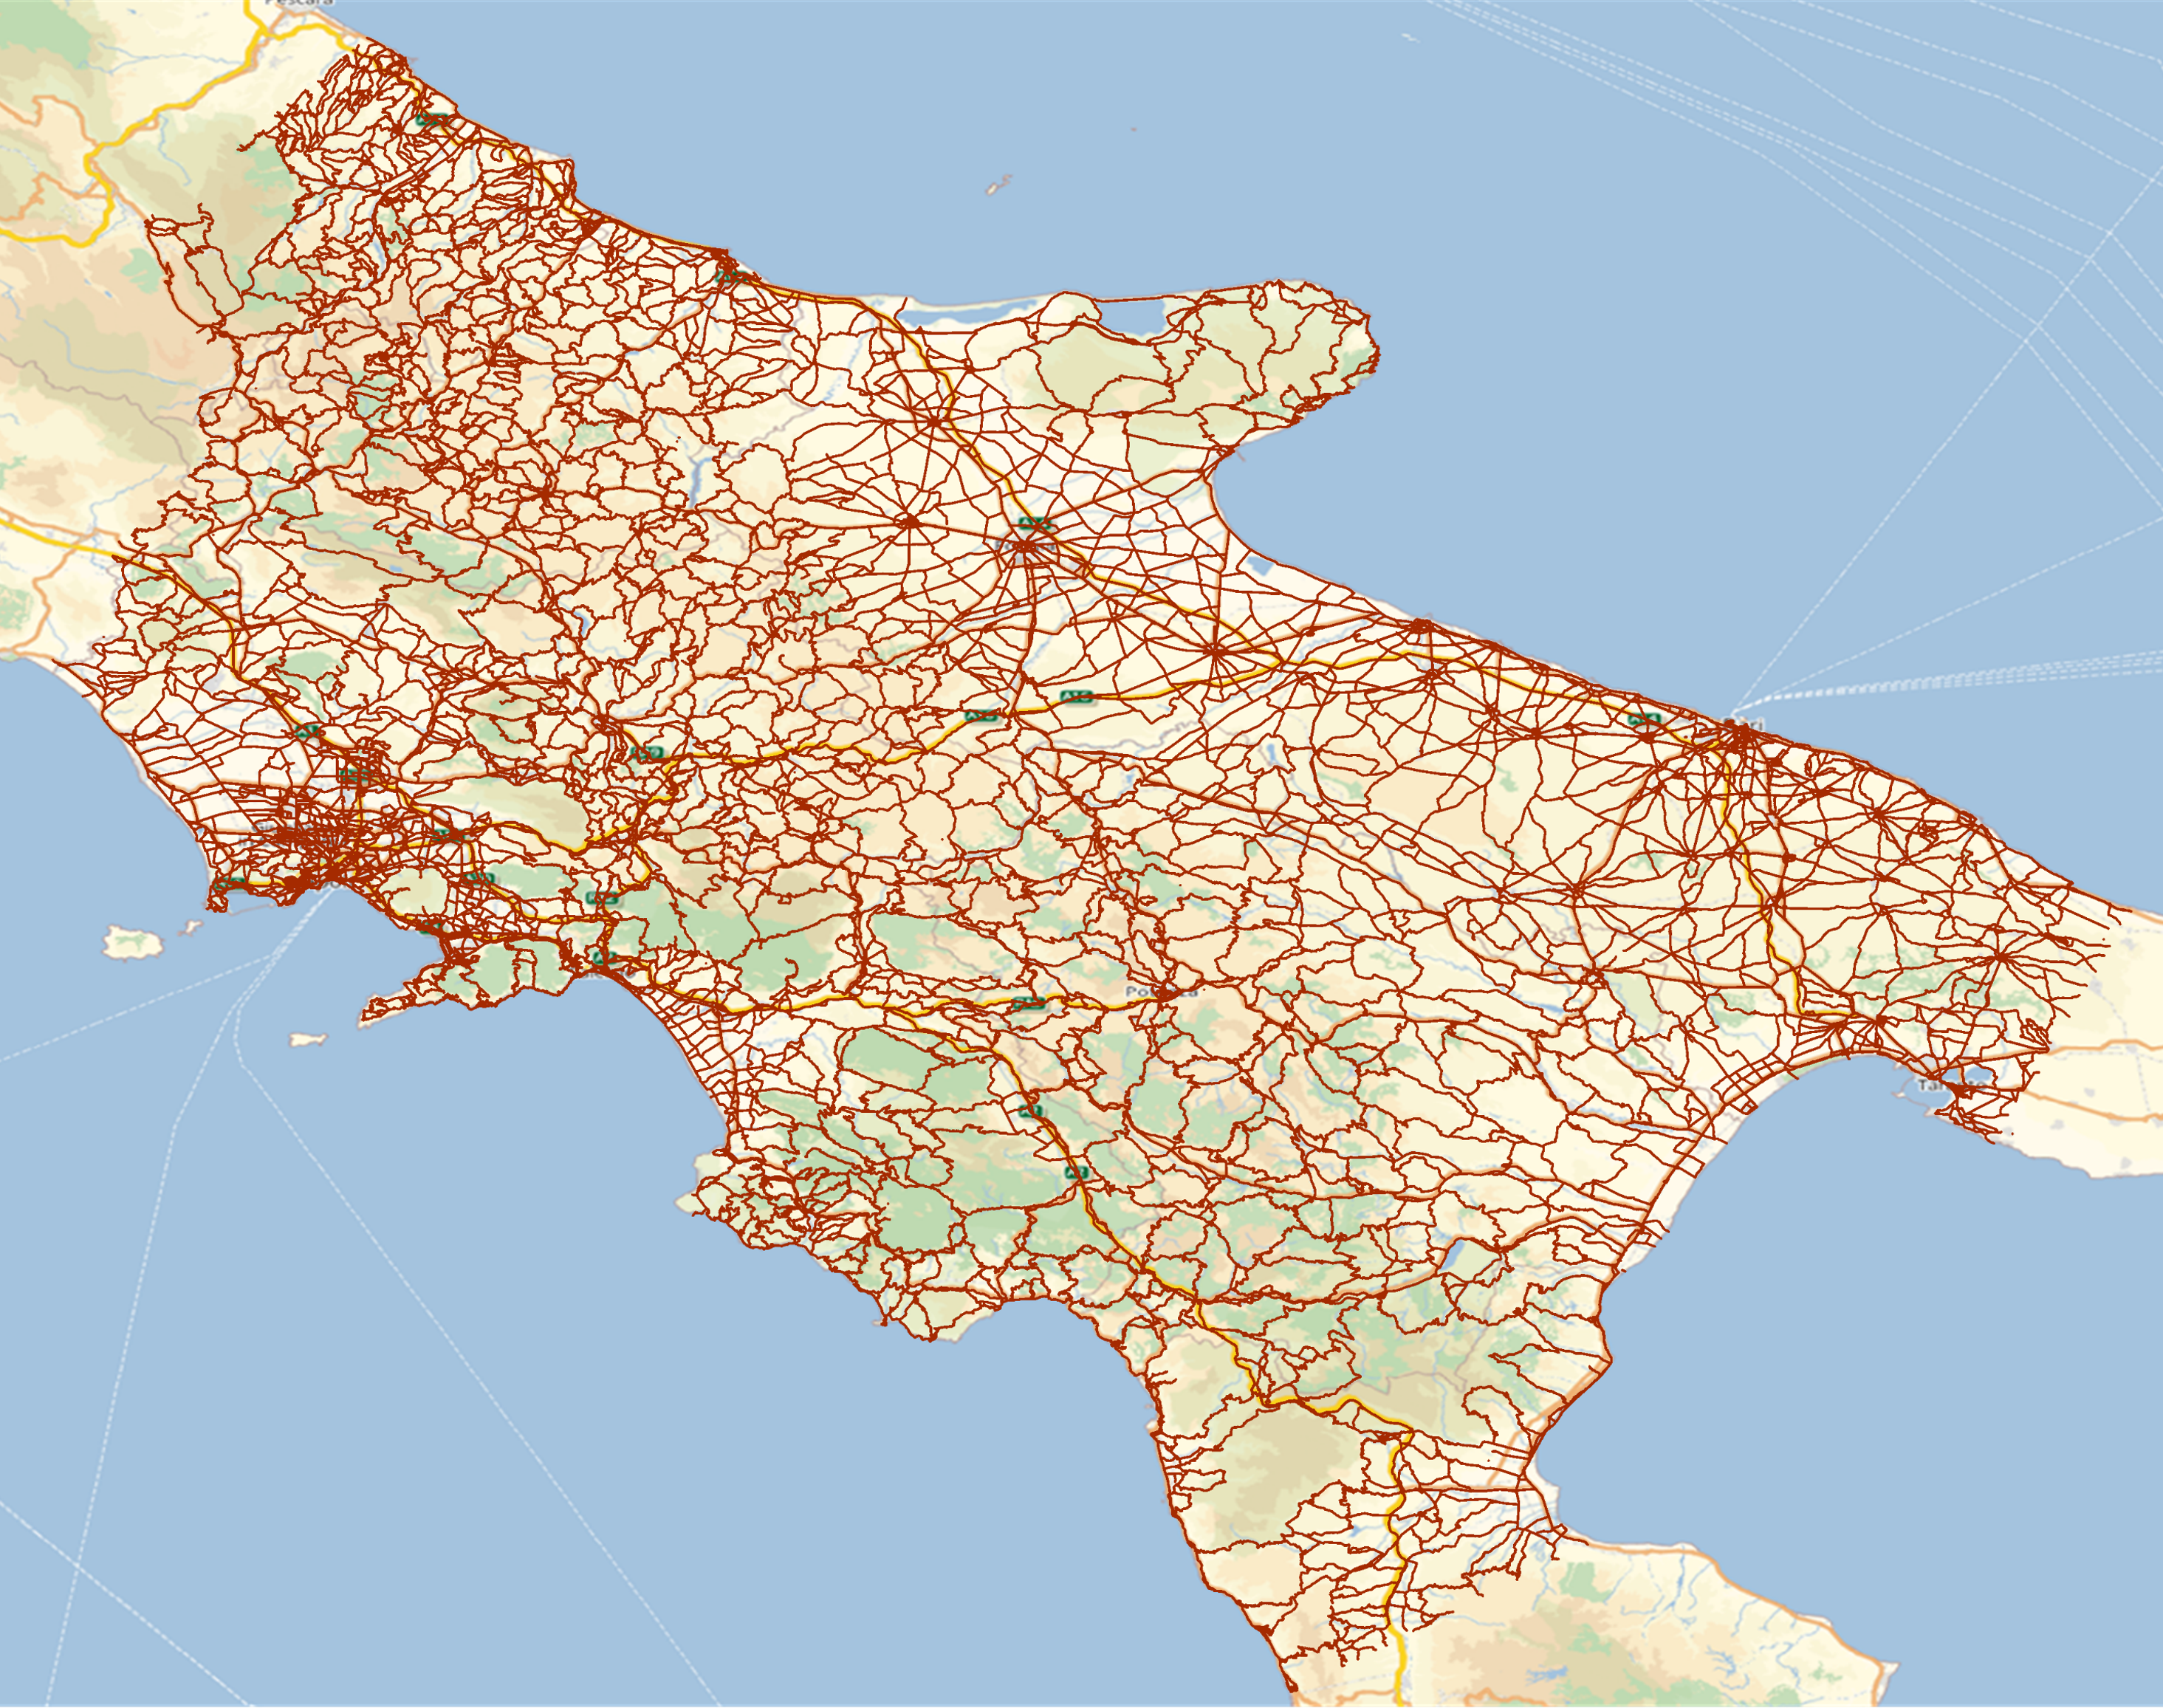
\includegraphics[width=.90\textwidth]{images/SupplyModel.png}}
    \caption{Supply Model for study area}
    \label{fig:supplymodel}
\end{figure}

\begin{figure}
\centering
{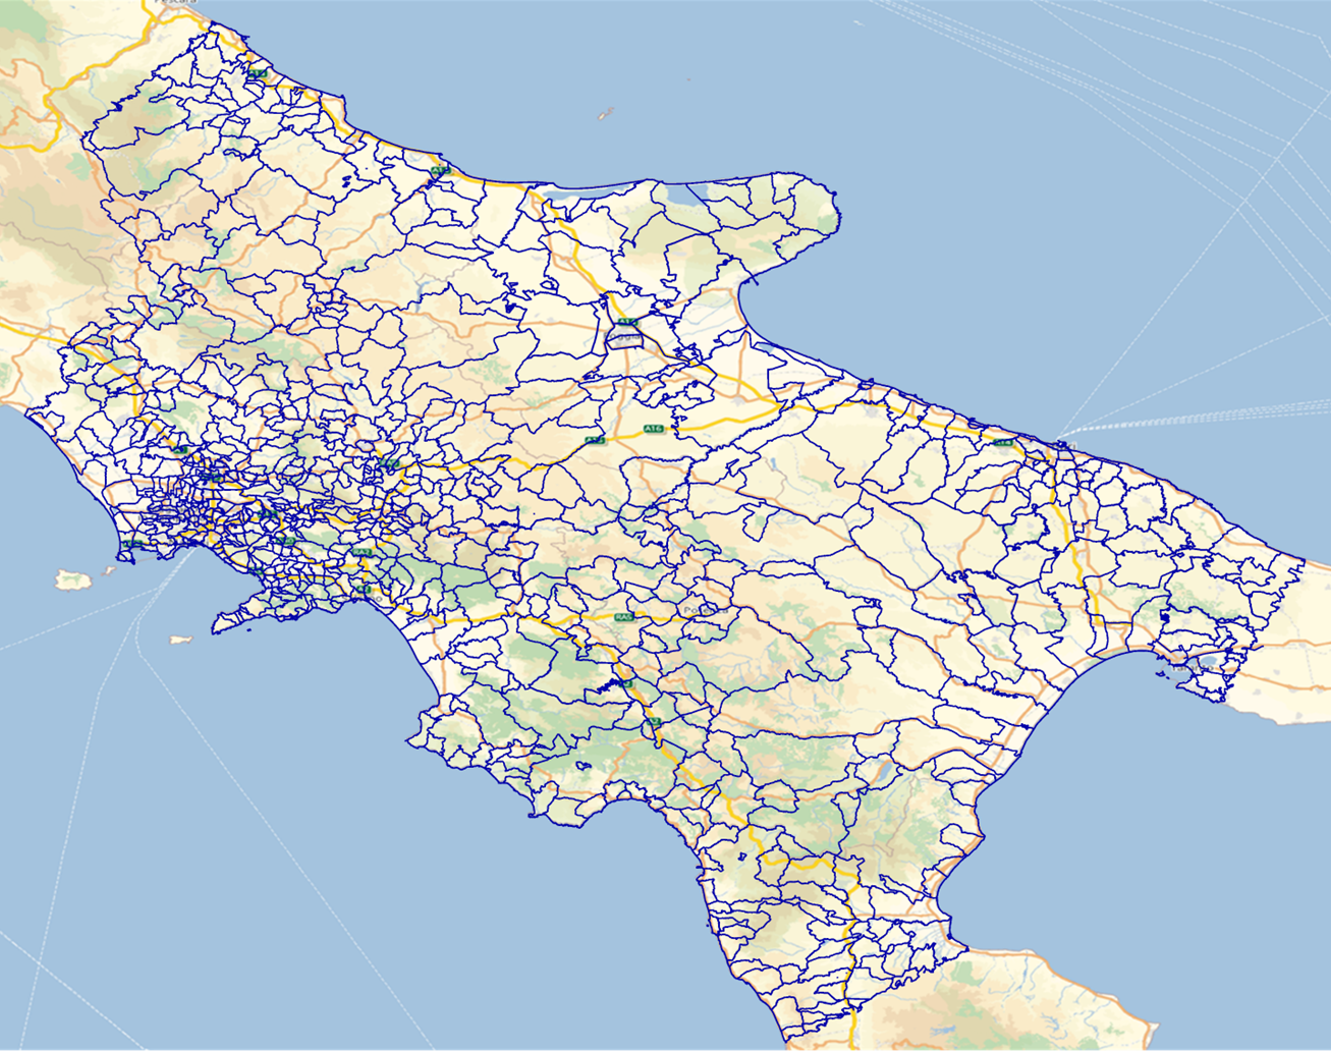
\includegraphics[width=.90\textwidth]{images/Zoning.png}}
    \caption{Zoning for study area}
    \label{fig:zoning}
\end{figure}

\section{Supply Model Development – Adjusting Free Flow Speeds in PTV Visum}
Accurate free-flow speed calibration is a critical aspect of transport modeling, ensuring that simulated traffic conditions reflect real-world driving behavior.Given the geographical and infrastructural characteristics of the Southern Italy study area, particularly in mountainous terrains and city centers, modifying the default speed limits in PTV Visum was necessary. Many tertiary and secondary roads had unrealistic speed limits (80–100 km/h), leading to inaccurate travel time estimations and unreliable network performance assessments. A systematic approach was implemented to filter, analyze, and reclassify road speeds based on road characteristics, naming conventions, and functional classifications.

\subsection{Identifying Misclassified Roads and Need for Speed Adjustments}
Upon importing the OpenStreetMap (OSM) road network into PTV Visum, initial observations revealed that many roads were assigned unrealistic speed limits. Mountainous roads, urban roads, and roads with high curvature often had speeds set at 80–100 km/h, which is not practical. Urban streets labeled “Via” or “Viale” had excessive speed limits, despite their functional characteristics suggesting lower speeds due to congestion, pedestrian activity, and intersections. Provincial and national roads (Provinciale, Statale) required further verification, as their design speeds varied significantly based on location and function. Since speed is a crucial factor in calculating shortest paths, travel times, and overall network efficiency, realistic speed calibration was necessary.

\subsection{Filtering and Reclassification Process in PTV Visum}
A structured approach was followed to identify and correct misclassified roads. First, tertiary and secondary roads with speeds between 80–100 km/h were extracted and manually reviewed. Each road segment was evaluated based on geometry, surrounding environment, and road naming conventions.\\
Curved, winding roads and irregular alignments were considered unsafe for high-speed driving and downgraded to 60 km/h where necessary. Urban roads, particularly those inside city centers, were reassigned 60 km/h speed limits, while highway-style rural roads with minimal intersections and wider lanes were preserved at higher limits. Roads labeled “Via” or “Viale” typically serve mixed-use areas with high pedestrian and vehicular interaction and were reclassified to 60 km/h. Provincial and national roads (Strade Provinciali - SP, Strade Statali - SS) were also reclassified: SP roads in urban/peri-urban areas were reduced to 60 km/h, while rural SP roads were kept at 90 km/h. SS roads were maintained at 90 km/h, depending on function and road width.\\
A final manual verification step was conducted, ensuring the new speed values matched real-world conditions. Road classifications were visually inspected in PTV Visum and compared with official Italian speed limits.

\subsection{Consideration of Road Characteristics and Functional Classes}
Beyond speed limits, additional factors were considered to improve model accuracy. Mountainous and hilly terrains were assigned lower speed classifications due to sharp turns and elevation changes. Roads with steep gradients and hairpin turns were reclassified to 60 km/h. High-traffic urban roads, even if categorized as secondary or tertiary roads, were also set at 60 km/h due to congestion.

\section{Validation of Speed Assumptions (Supply Model Validation)}
\subsection{Selection of Origin-Destination (OD) Pairs}
A total of 84 OD pairs were chosen across 58 zones to encompass diverse regions and travel conditions reported in \ref{fig:zones modelvalidation}. This included 18 OD pairs from provincial capitals to ensure a mix of urban and interregional routes. Additional OD pairs were strategically placed to cover different road types, variations in free-flow speed, and locations between seismic faults to assess network resilience.
The comparison has been made on uncongested travel time using data obtained by Google Maps (that represent our real data) and the ones obtained by the model. The data collected by Google used a query where the starting time was settled at 1–2 AM to ensure minimal congestion effects, aligning with the model's free-flow conditions

\begin{figure}
\centering
{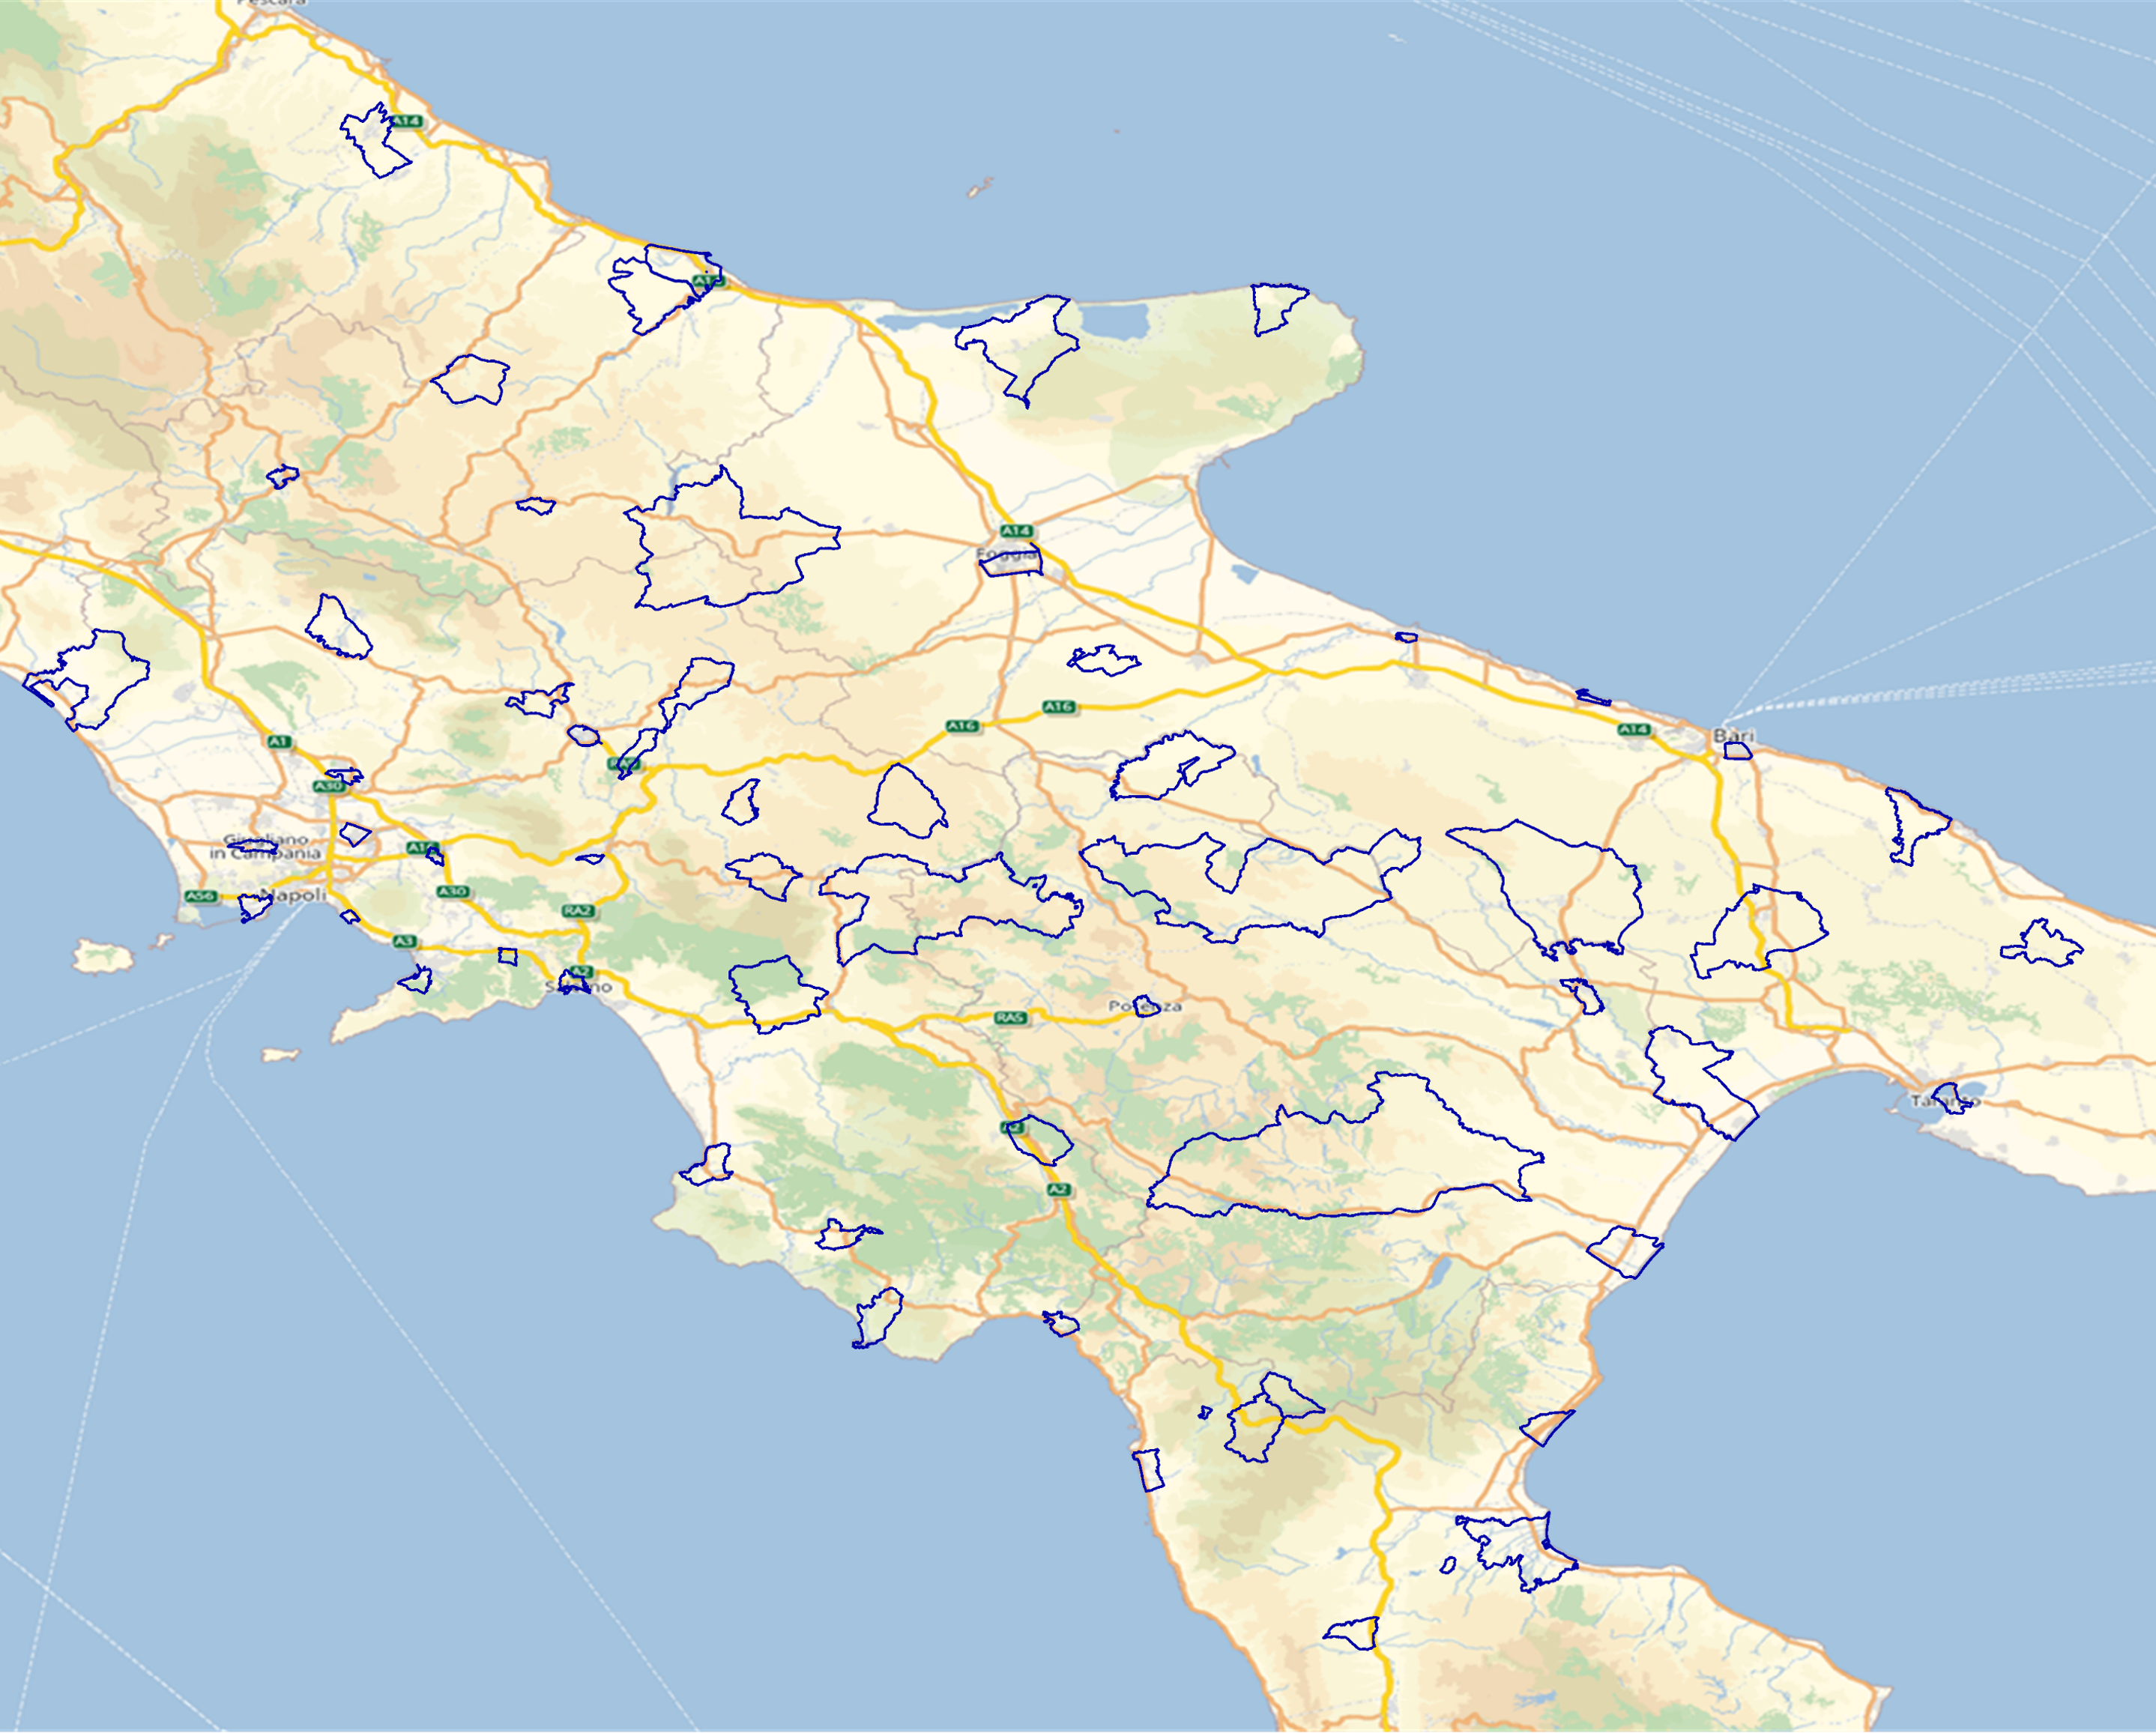
\includegraphics[width=.8\textwidth]{images/Validation_zones.png}}
    \caption{Zones used for validating the model}
    \label{fig:zones modelvalidation}
\end{figure}

\subsection{Data Analysis and Validation Results}
A scatter plot was generated to compare travel times from PTV Visum with those from Google Maps. Linear regression analysis yielded the equation:
\begin{equation}
y = 0.9684x + 5.9104
\end{equation}

where \( y \) represents PTV Visum travel time and \( x \) represents Google Maps travel time. The coefficient (0.9684) indicated that PTV Visum travel times were closely aligned with real-world data, and an \( R^2 \) value of 0.9779 confirmed strong correlation.Most OD pairs had errors within $\pm 10$--$15\%$, which was within an acceptable validation range. A few outliers with deviations above $20\%$ indicated potential local variations in speed assumptions.
A graphical representation of regression are shown in 

\begin{figure}
\centering
{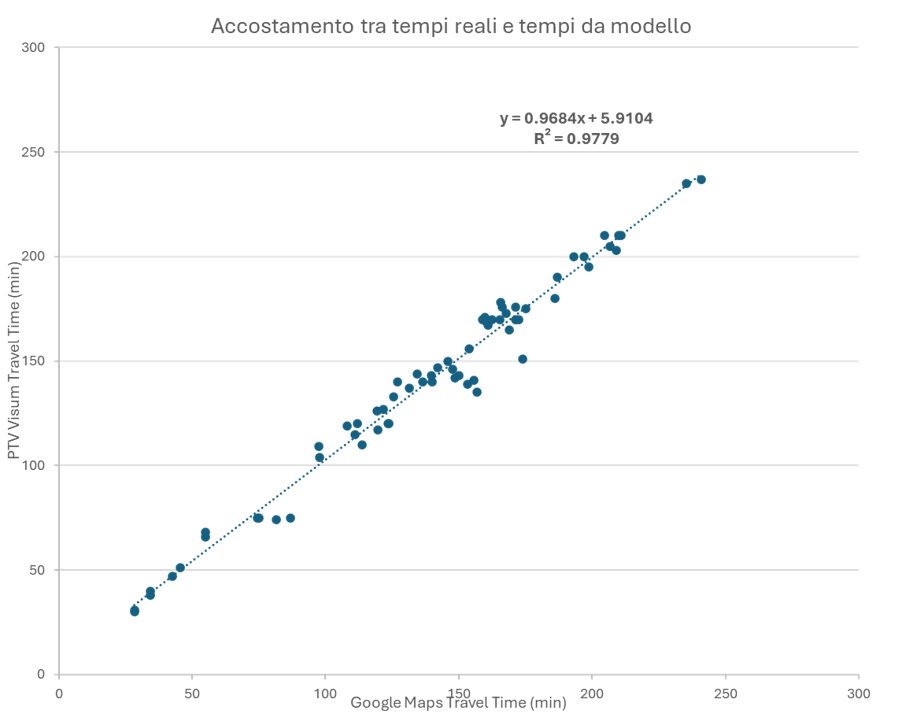
\includegraphics[width=.8\textwidth]{images/Validation_results.png}}
    \caption{$R^2$ between uncongested travel time}
    \label{fig:modelvalidation}
\end{figure}

\subsection{Implications of Speed Adjustments for the Supply Model}
By refining free-flow speeds, the transport model in PTV Visum now provides:
\begin{itemize}
    \item More realistic travel times, improving the accuracy of traffic assignment models.
    \item Better route selection behavior, reducing overestimation of highway usage in mountainous and urban areas.
    \item Stronger validation with real-world data, ensuring network performance indicators (e.g., betweenness centrality, connectivity, and redundancy) are correctly represented.
\end{itemize}

\section{Seismic Disruption Scenarios and Network Impact Analysis}

Assessing the impact of seismic events on transportation networks is crucial for understanding network resilience and planning effective mitigation strategies. In this context, redundancy indicators such as the beta index, gamma index, betweenness centrality, average degree, and clustering coefficient are essential metrics that provide insights into network connectivity, complexity, and robustness. This section outlines the methodology used to model seismic disruptions, evaluate their effects on the transport network, and analyze key resilience indicators.

\subsection{Seismic Fault Impact Scenarios}

To assess the impact of seismic events on the transport network, two disruption scenarios were defined for each of the three identified seismic fault points in Southern Italy. These scenarios were designed to represent varying levels of earthquake intensity and their corresponding effects on road infrastructure.

The disruption scenarios were defined as follows:
\begin{itemize}
    \item \textbf{Low-intensity earthquake}: 10 percent of road links within an 8 km radius of the fault point were disrupted.
    \item \textbf{High-intensity earthquake}: 40 percent of road links within a 15 km radius of the fault point were disrupted.
\end{itemize}

To identify affected road links, QGIS spatial analysis was used to create buffer zones of 8 km and 15 km radii around each seismic fault point. All road links within these buffer zones were extracted, and a random selection process was applied to disrupt 10 percent of links in the low-intensity scenario and 40 percent in the high-intensity scenario. This random selection simulates the unpredictable nature of earthquake-induced infrastructure failures.

These selected disrupted links were then imported into PTV Visum for network disruption modeling. In PTV Visum, disruptions were applied by setting the capacity (CapPrT) of the affected links to 0, simulating their failure and removal from the network. This process allowed for the assessment of network performance under earthquake conditions, identifying changes in connectivity, alternative routing possibilities, and potential congestion zones.



\chapter{Results and Discussion}

\section{Introduction}
This chapter presents the results of the network resilience analysis by examining how seismic disruptions impact key transport network indicators. The findings are based on the betweenness centrality, beta index, gamma index, clustering coefficient, average degree, and redundancy indicator before and after disruption scenarios. By comparing these indicators, the chapter highlights how different road classifications and regional transport networks respond to disruptions, identifying the most vulnerable areas and critical links in Southern Italy.

The results are structured as follows: First, the general network indicators before and after disruption are presented, summarizing key trends and observations. Then, a detailed analysis of each indicator is provided, including percentage changes and their significance in assessing network resilience. The discussion focuses on identifying critical links and evaluating the degree of connectivity loss due to seismic events.

The first part of this analysis focuses on betweenness centrality, a key measure that identifies the most important road segments in facilitating movement across the transport network. The evaluation of critical road links before and after disruption provides insight into how seismic events redistribute traffic flow and increase congestion in alternative routes.

\section{Betweenness Centrality of Links Before and After Disruption}
Betweenness centrality is a fundamental measure in transport network analysis, representing the extent to which a link is used in the shortest paths across the network. Links with high betweenness centrality serve as major traffic conduits, meaning their failure would significantly impact regional connectivity. This section evaluates betweenness centrality before and after disruption, highlighting critical road links and the impact of seismic faults.

\subsection{Betweenness Centrality Before Disruption (Business-As-Usual Scenario)}

In the BAU scenario, the transport network operates without disruptions, meaning that betweenness centrality is distributed based on natural travel demand patterns and existing road capacities. The graphical representation of betweenness centrality in this scenario highlights the most important links for regional and interregional transport.

The network is classified into four categories based on betweenness centrality values:

\begin{itemize}
    \item \textbf{Red links (1.5\%)} are the most critical links, experiencing the highest level of centrality. These links are heavily concentrated around seismic faults 1 and 2, particularly in Campania, where primary road corridors support significant traffic flows.
    \item \textbf{Yellow links (10.5\%)} are high-importance links, mainly consisting of motorways and primary roads that provide essential long-distance connectivity.
    \item \textbf{Green links (35\%)} are moderately important routes, often serving as secondary alternatives to the primary road network.
    \item \textbf{Black links (53\%)} are the least critical, comprising rural, local, or low-traffic roads that contribute minimally to shortest-path flows.
\end{itemize}

The mean betweenness centrality in the BAU scenario is \textbf{0.0047}, with a standard deviation of \textbf{0.0020}, reflecting a network where a few highly centralized corridors dominate overall connectivity.

\subsection{Regional Differences in Betweenness Centrality Before Disruption}

The spatial distribution of high-centrality links varies significantly across different regions:

\textbf{Campania}, located in the western part of the study area, contains the highest concentration of red and yellow links, meaning that disruptions in this region would cause severe network fragmentation and increased travel times. This region serves as a key economic and transport hub, reinforcing the high reliance on major corridors.

\textbf{Puglia} exhibits a more balanced centrality distribution, with fewer red links and a greater proportion of yellow and green links. This indicates that Puglia’s network structure provides more redundancy and flexibility, making it moderately resilient to disruptions.

\textbf{Calabria}, particularly around Seismic Fault 3, has fewer high-centrality links, indicating that disruptions in this area would have a limited impact on overall network performance. The regional road network is less centralized, reducing the reliance on individual corridors.

These differences suggest that not all regions experience the same level of vulnerability, with Campania being the most critical, followed by Puglia, and Calabria being the least affected in a pre-disruption scenario.

\begin{figure}[H]
\centering
{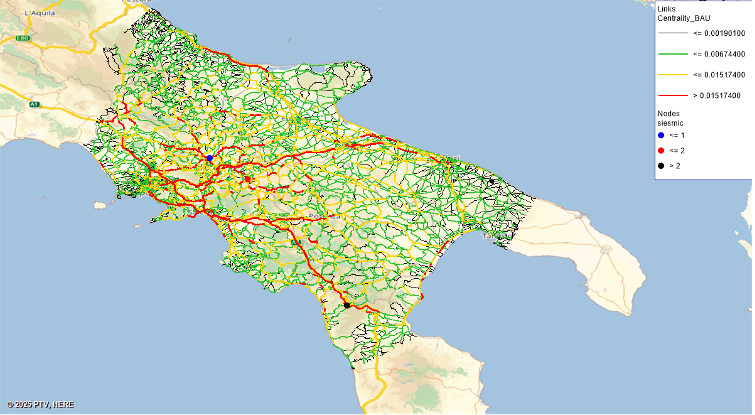
\includegraphics[width=1\textwidth]{images/Picture 1.png}}
    \caption{Betweenness Centrality of links ( BAU ) }
\end{figure}

\subsection{Changes in Betweenness Centrality After Disruption}
To assess how seismic events impact network connectivity, betweenness centrality was recalculated for six seismic fault scenarios. The analysis measures how critical link distributions change post-disruption and which road segments become more dominant in shortest-path calculations due to rerouting effects.

The table below summarizes the percentage change in the number of links classified as Red, Yellow, Green, and Black compared to the BAU scenario.

  \begin{table}[H]
\centering
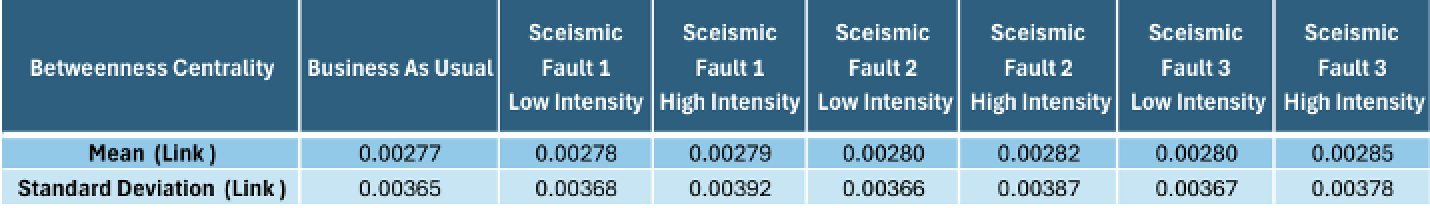
\includegraphics[width=\textwidth]{images/Table1.png}
\caption{Mean and Standard Deviation of Betweenness Centrality of Links}
\label{tab:betweenness_stats}
\end{table}

  \begin{table}[H]
\centering
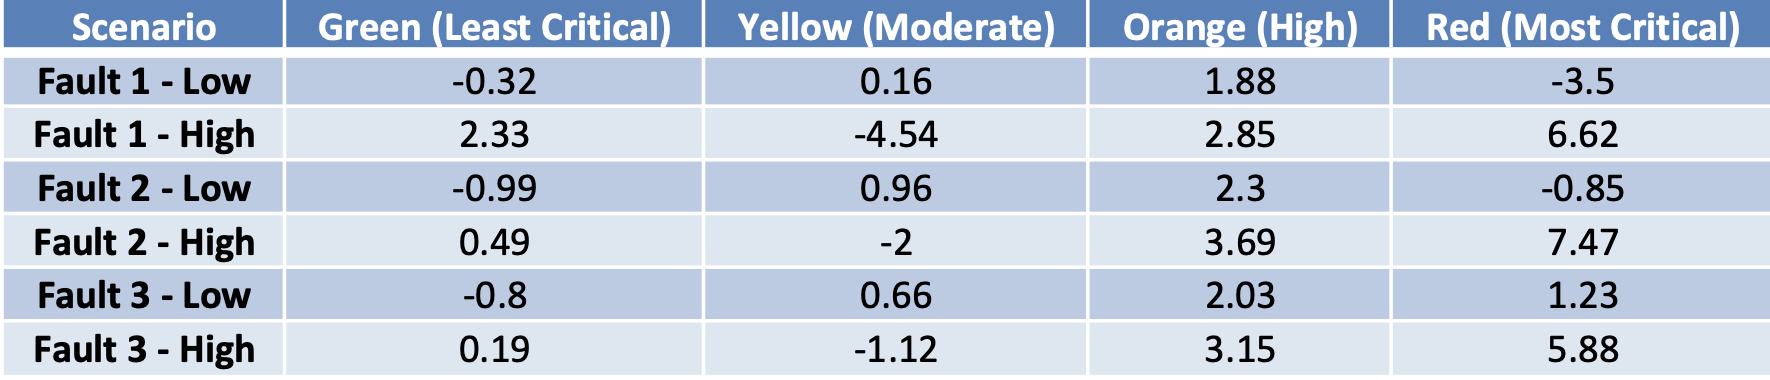
\includegraphics[width=\textwidth]{images/Table2.png}
\caption{Classification of Betweenness Centrality of Links}
\label{tab:classification_fault1}
\end{table}


The results indicate that Seismic 1 and 2 at the 15km buffer level cause the most severe shifts, with red links increasing by more than 6.5 percent, indicating new congestion points forming due to rerouted traffic. The greatest reductions in green links occur in Seismic 1 (15km) (2.33 percent), showing that some previously important secondary roads lost their significance after disruption.

Seismic Fault 3, particularly in the 15km scenario, sees a +5.88 percent increase in red links, meaning that some roads in Calabria gained importance, though not as significantly as in Campania. This suggests that while Calabria’s road network is generally less vulnerable, large-scale disruptions can still shift network reliance onto specific corridors.

These shifts in betweenness centrality confirm that primary roads (motorways and key interregional routes) become even more critical post-disruption, requiring strategic planning to mitigate congestion and maintain accessibility.

\subsection{Interpretation and Discussion of Results}
The betweenness centrality results reveal significant shifts in network criticality across different seismic scenarios. The analysis shows that the average betweenness centrality values decrease as seismic intensity increases, indicating that fewer links maintain high importance in shortest-path calculations post-disruption. The standard deviation values also decrease, suggesting that centrality values become more evenly distributed across the network, making it less centralized around key corridors.

The Business-As-Usual (BAU) scenario shows the highest average centrality at 0.00277, with a standard deviation of 0.00365, reflecting a network where a few highly centralized corridors dominate overall connectivity. As disruptions increase, centrality values decline, with the most significant drop occurring in Seismic 2 - High (0.00282 Mean, 0.00387 Std Dev), highlighting the severe impact of this disruption on network connectivity.

Campania remains the most vulnerable region, as it has the highest number of red and yellow links, meaning disruptions in this area cause widespread traffic shifts. Motorways continue to play a dominant role in connectivity, but seismic events increase reliance on secondary roads, which may not be designed to handle heavy rerouted traffic. Calabria remains relatively stable, reinforcing that its road network is less centralized and less dependent on a few critical links.

Seismic Fault 1 and Seismic Fault 2 create the highest impact, while Fault 3 disruptions are less significant. In large-scale disruptions (15km buffer), Seismic Fault 3 sees a noticeable increase in red links, suggesting that while Calabria is generally less vulnerable, major disruptions can still cause new bottlenecks to form.

By integrating these findings with the classification of links into Red, Yellow, Green, and Black, it becomes clear that seismic disruptions do not affect all roads equally. High-betweenness links are concentrated around Campania, confirming its importance as a key transport hub, while Calabria's dispersed network structure makes it more resilient in smaller-scale disruptions.

\subsection{Implications for Seismic Resilience and Conclusion}
The results highlight the need for targeted strategies to improve network resilience in earthquake-prone areas. Major motorways (yellow links) require reinforcement to prevent excessive strain on alternative routes when disruptions occur. The findings confirm that Campania is the most vulnerable region, requiring redundancy strategies such as alternative expressways and reinforced detour routes to ensure minimal disruptions.

The analysis also demonstrates that secondary roads(green links)fluctuate in importance post-disruption, meaning that alternative routing strategies should focus on preserving connectivity in high-betweenness areas near Fault 1 and Fault 2.

Betweenness centrality analysis provides a clear understanding of how the transport network adapts to seismic disruptions. By prioritizing the most affected areas, resilience strategies can be tailored to mitigate congestion, enhance redundancy, and ensure faster recovery after seismic events. These findings reinforce the importance of strengthening primary corridors and ensuring that secondary roads are adequately integrated into post-disruption traffic management plans.

\section{Node Betweenness Centrality Analysis}
Betweenness centrality for nodes provides insights into how crucial intersections and junctions are within the transport network. Nodes with high betweenness centrality act as critical connectors, facilitating traffic movement across the network. This section examines betweenness centrality in the Business-As-Usual (BAU) scenario and evaluates changes following seismic disruptions.

\subsection{Business-As-Usual (BAU) Scenario}
Before disruptions, node betweenness centrality was highest along motorways and trunk roads, particularly in \textbf{Campania (Fault 1)} and \textbf{Apulia (Fault 2)}. These regions serve as primary transport corridors, connecting urban and rural areas. The graphical representation of the Business-As-Usual (BAU) scenario indicates that:

\begin{itemize}
    \item \textbf{Most red nodes} (high centrality) are concentrated along major highways, motorways, and trunk roads.
    \item \textbf{Yellow and orange nodes} are found in secondary and tertiary roads, playing a supporting role in connectivity.
    \item \textbf{Green nodes}, which represent the lowest centrality values, dominate rural and less-connected areas.
\end{itemize}

The mean betweenness centrality for the BAU scenario was \textbf{0.004147}, with a standard deviation of \textbf{0.004700}, indicating a wide variability in node importance across the network.

\begin{figure}[H]
\centering
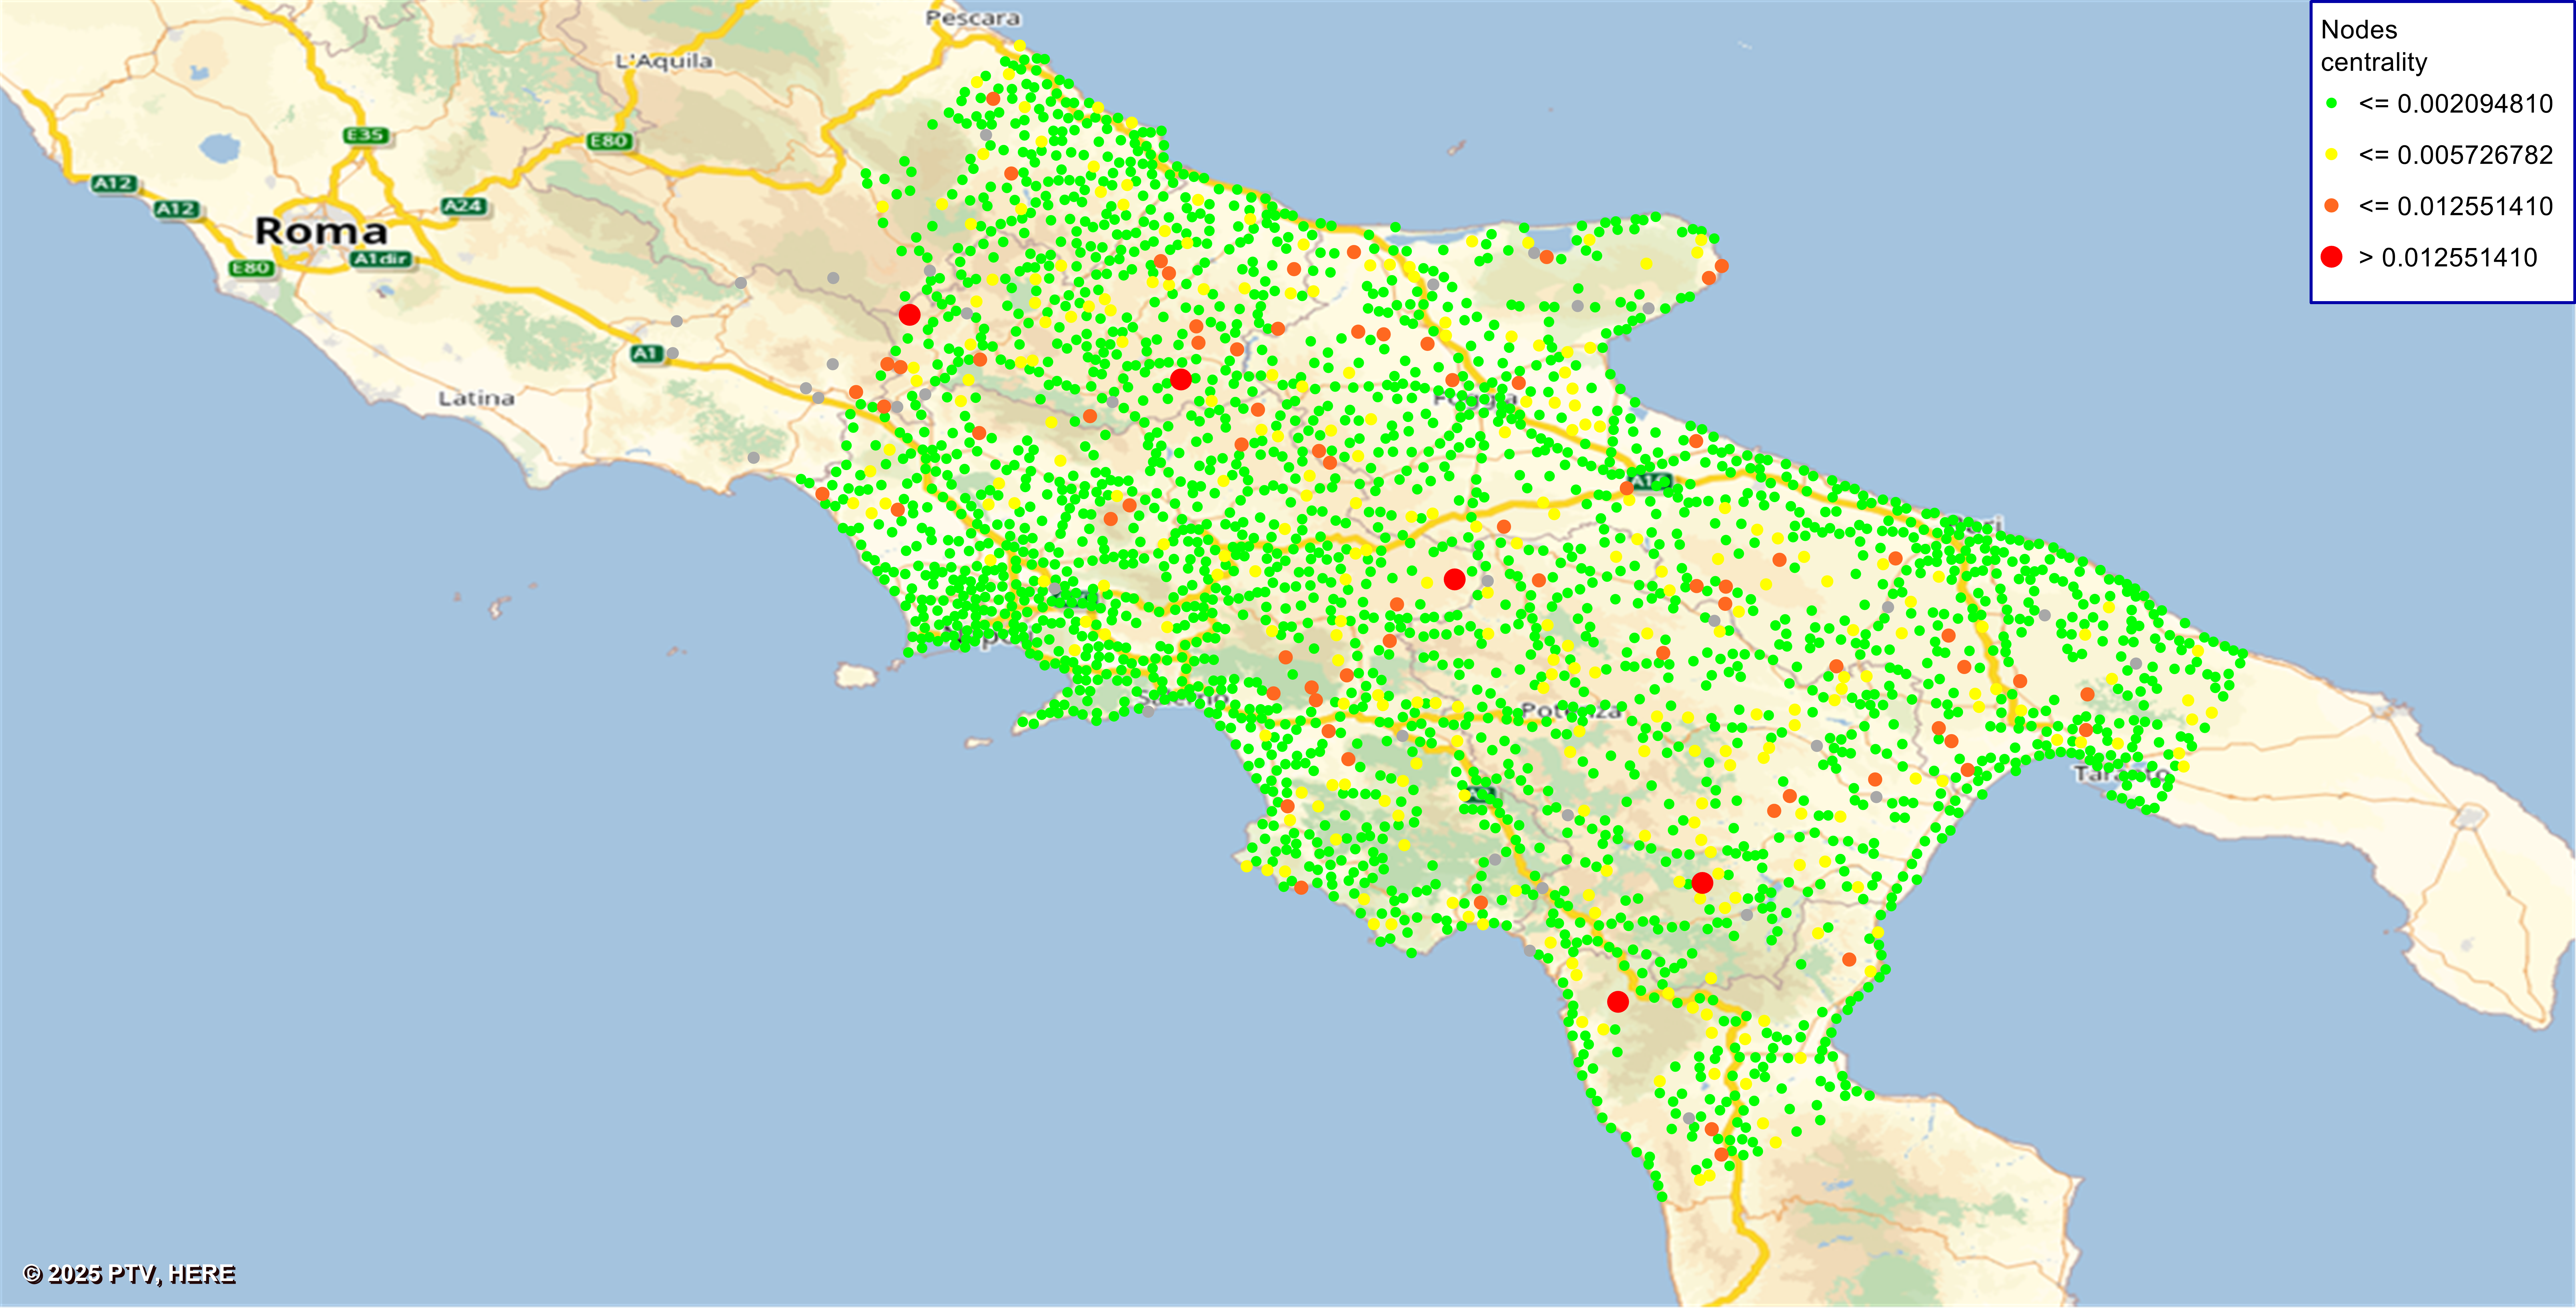
\includegraphics[width=1\textwidth]{images/Centrality_BAU_node 2.png}
\caption{Node Betweenness Centrality in BAU Scenario (Graphical Representation)}
\label{fig:bau_node_centrality}
\end{figure}


   \subsection{Changes in Betweenness Centrality After Disruption}
   After seismic disruptions, the mean and standard deviation of betweenness centrality shifted across all scenarios, reflecting the changes in network connectivity due to road failures.

 \begin{table}[H]
\centering
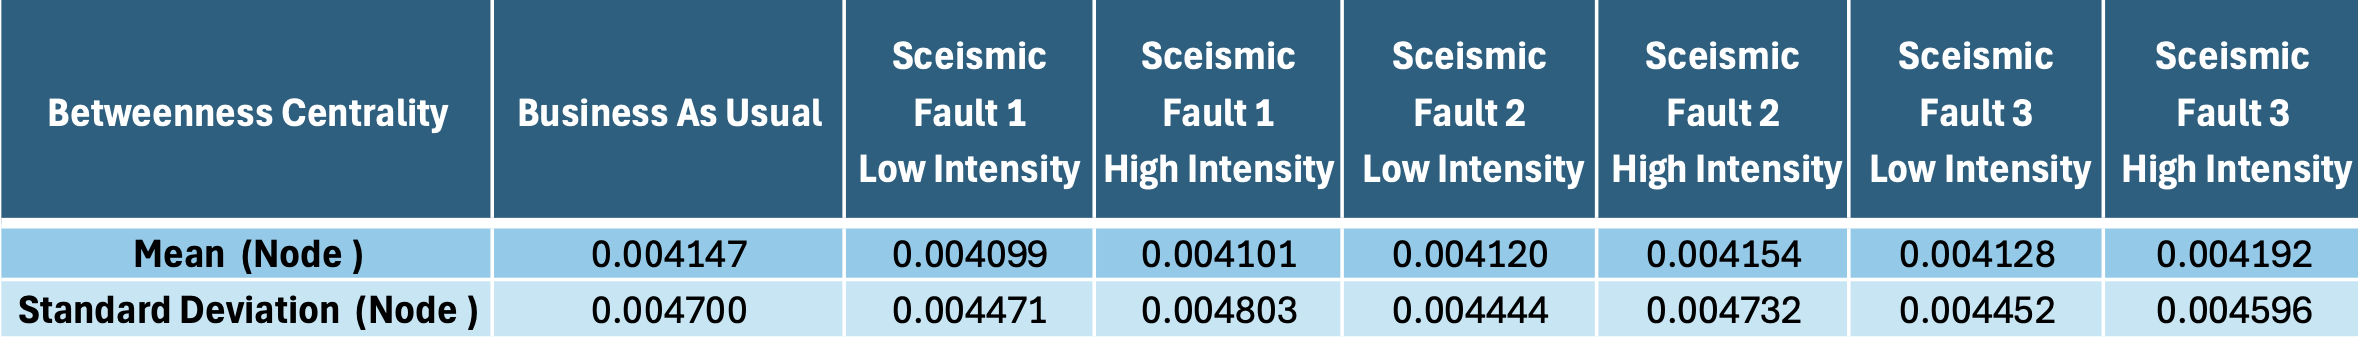
\includegraphics[width=1\textwidth]{images/Table3.png}
\caption{Mean and Standard Deviation of Node Betweenness Centrality Before and After Disruption.}
\label{tab:node_centrality_change}
\end{table}

\textbf{Key Observations}
\begin{itemize}
    \item Minor shifts in mean centrality indicate that the core network structure remains intact, but significant redistribution of centrality values occurs at a local level.
    \item \textbf{Seismic Fault 3 - High Intensity} had the highest mean increase (\textbf{0.004192}), indicating that critical nodes in Calabria became more central after disruption.
    \item Standard deviation increased in most high-intensity scenarios, signifying higher disparities in node importance, as some intersections gained significance while others lost connectivity.
\end{itemize}

 \begin{table}[H]
\centering
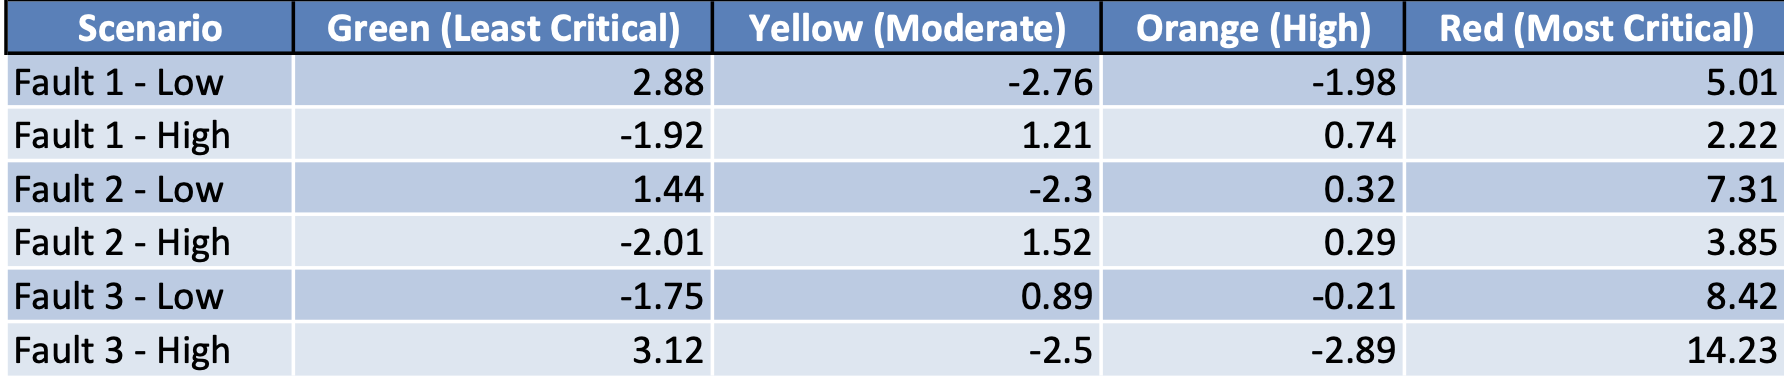
\includegraphics[width=1\textwidth]{images/Table4.png}
\caption{Percentage Change in Node Centrality Categories}
\label{tab:node_centrality_change_categories}
\end{table}

\subsection{Interpretation of Results}
\begin{itemize}
    \item \textbf{Fault 3 - High Intensity} produced the highest increase in red nodes (\textbf{+14.23\%}), significantly impacting network flow.
    \item \textbf{Fault 1} and \textbf{Fault 2} had lower but still notable increases in critical nodes, ranging between \textbf{+3.85\%} and \textbf{+7.31\%}.
    \item \textbf{Green (least critical)} nodes fluctuated across scenarios, but major shifts occurred in \textbf{red (most critical)} and \textbf{yellow (moderate)} nodes.
    \item \textbf{Yellow nodes} decreased in most scenarios, indicating that some moderately important nodes lost significance as traffic concentrated on a smaller set of high-betweenness intersections.
\end{itemize}

\subsection{Regional Differences and Seismic Fault 3’s Impact}
Although Fault 3 was initially the least critical area before the earthquake, it became the most affected after seismic events due to its lower number of nodes (intersections) and reduced network redundancy. This structural limitation made it highly vulnerable to disruptions, leading to the highest increase in critical nodes.

\textbf{Comparison Across Faults:}
\begin{itemize}
    \item \textbf{Fault 1 (Campania)} and \textbf{Fault 2 (Apulia)} had higher pre-disaster redundancy, distributing traffic shifts more evenly across the network.
    \item \textbf{Calabria (Fault 3)} had fewer alternative paths, making each disruption more impactful.
    \item \textbf{Seismic Fault 1} and \textbf{Fault 2} had smaller shifts in centrality values, reinforcing their robustness compared to Calabria.
\end{itemize}

\textbf{Implications for Seismic Resilience Planning:}
\begin{itemize}
    \item \textbf{Calabria} requires targeted infrastructure investments to enhance redundancy.
    \item \textbf{Traffic management strategies} should prioritize maintaining alternative routes in regions with fewer intersections.
    \item \textbf{Betweenness centrality shifts} indicate that post-earthquake detour planning must account for regions where minor disruptions cause large-scale bottlenecks.
\end{itemize}

\textbf{Final Takeaway}

Betweenness centrality analysis demonstrates that seismic events not only create new critical nodes but also significantly reshape the network hierarchy. While Campania and Apulia remained major transport corridors before and after seismic disruptions, Calabria's role changed significantly, evolving from a low-impact region to the most vulnerable in high-intensity scenarios. These findings highlight the necessity of pre-disaster planning to reinforce transport networks in low-density regions and ensure long-term resilience.

\section{Beta Index Analysis}
\subsection{Beta Index Before Disruption (BAU)}
The beta index measures network complexity by quantifying the ratio of links to nodes in the transport network. A higher beta index indicates a more interconnected and resilient network, while a lower beta index suggests a sparser network with fewer available alternative routes.

In the Business-As-Usual (BAU) scenario, the beta index is 1.4676, indicating a well-connected network with sufficient link redundancy. This suggests that under normal conditions, the transport network in Southern Italy provides multiple pathways for connectivity.

\subsection{Beta Index Changes After Disruption}
Following seismic disruptions, the beta index experienced minor variations across different earthquake scenarios. The table below summarizes the beta index values before and after disruptions, along with the percentage changes:

\begin{table}[H]
\centering
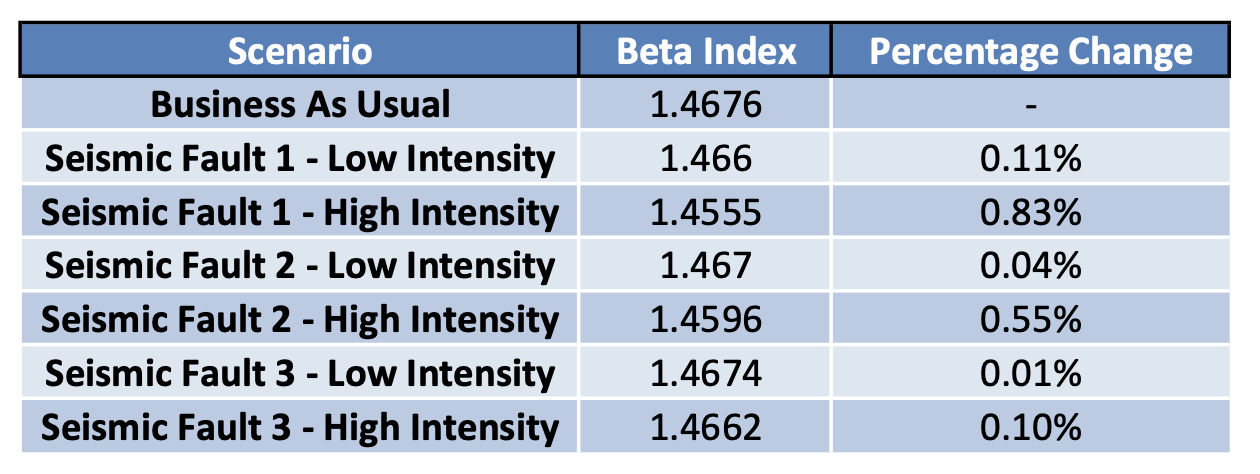
\includegraphics[width=1\textwidth]{images/Table5.png}
\caption{Beta Index Values and Percentage Change Across Seismic Disruption Scenarios}
\label{tab:beta_index_change}
\end{table}

The most significant drop in beta index occurred in Seismic Fault 1 - High Intensity (-0.83\%), indicating that this region experienced the greatest network fragmentation. This decline suggests a reduction in alternative routes due to road failures. Similarly, Seismic Fault 2 - High Intensity (-0.55\%) also exhibited a notable decrease, highlighting disruptions in this region.

Conversely, the Seismic Fault 3 scenarios showed minimal reductions in beta index (-0.01\% to -0.10\%), reinforcing that this region was initially less connected and therefore experienced fewer changes in network complexity.

\subsection{Interpretation of Results}
Seismic Fault 1 experienced the highest decrease in beta index, reflecting a greater disruption impact in this region. Seismic Fault 2 also showed a noticeable decline, indicating significant disruptions but with slightly better connectivity retention than Fault 1. Seismic Fault 3 remained relatively stable, suggesting that this region had fewer alternative links to begin with, making its overall network complexity less affected. Although all scenarios experienced some reduction in the beta index, the changes were minor, indicating that despite disruptions, the transport network maintains a reasonable level of connectivity.

\subsection{Implications for Seismic Resilience}
Regions with higher beta index reductions, such as Fault 1 and Fault 2, need targeted interventions like road reinforcements and redundancy planning. Alternative route planning should focus on areas where connectivity dropped the most, ensuring continued mobility after seismic events. Minimal beta index changes in Fault 3 indicate a pre-existing sparsity in the network, requiring long-term infrastructure planning rather than short-term resilience strategies.

This analysis provides a foundational understanding of how seismic events impact overall network complexity and highlights the importance of designing resilient road infrastructures that minimize connectivity losses.

\section{Gamma Index (Planar Coefficient) Analysis}
\subsection{Planar Coefficient Before Disruption (BAU)}
The gamma index (planar coefficient) measures the degree of connectivity within a transport network, specifically in planar networks such as road systems, where links are constrained by geographical and physical layout restrictions. A higher gamma index indicates a well-connected network with multiple route options, while a lower gamma index suggests a more fragmented or sparse network.

In the Business-As-Usual (BAU) scenario, the planar coefficient is 0.4892, suggesting that the Southern Italy transport network has a moderate level of connectivity, with some redundancy in routes but also certain constraints that limit the overall connectivity potential.

\subsection{Changes in Planar Coefficient After Disruption}
Seismic events impact the gamma index by disrupting road links, reducing the number of possible connections, and forcing traffic onto fewer alternative paths. The table below summarizes the planar coefficient before and after seismic disruptions, along with the percentage change for each scenario.

\begin{table}[H]
\centering
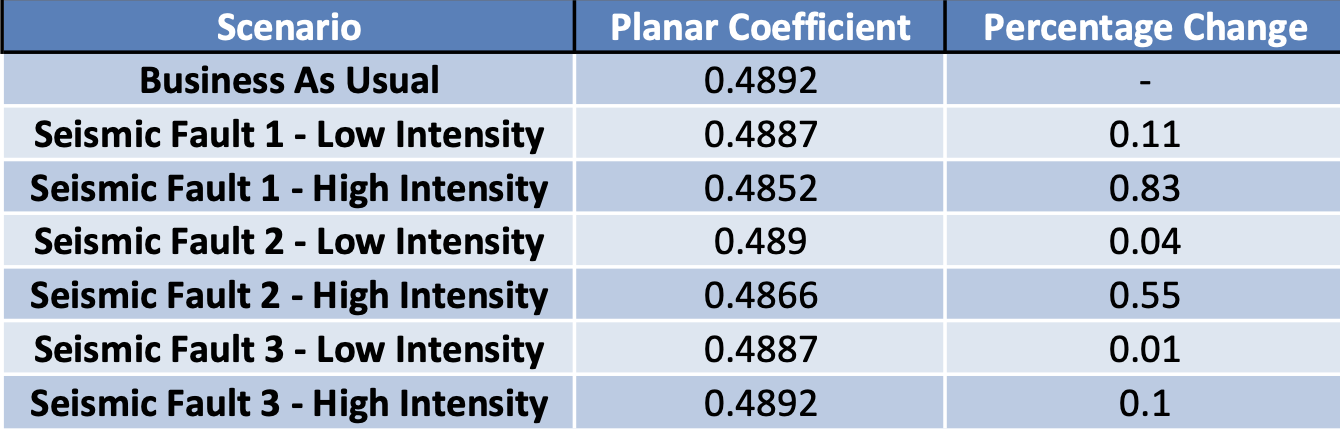
\includegraphics[width=1\textwidth]{images/Table6.png}
\caption{Planar Coefficient Values and Percentage Change Across Seismic Scenarios}
\label{tab:planar_coefficient_change}
\end{table}

The most significant drop in the gamma index occurred in Seismic Fault 1 - High Intensity (-0.83\%), indicating that this scenario caused the greatest disruption in connectivity. This reduction suggests that a higher number of links were lost or became non-functional, leading to a reduction in network-wide accessibility.

Seismic Fault 2 - High Intensity also exhibited a noticeable decrease of -0.55\%, confirming that this region also experienced significant connectivity disruptions. In contrast, Seismic Fault 3 scenarios showed minimal reductions (-0.01\% to -0.10\%), suggesting that the initial network configuration in this region was already sparse, and disruptions had a lower relative impact.

\subsection{Interpretation of Results}
Seismic Fault 1 experienced the highest reduction in gamma index, which means the region suffered from the greatest connectivity loss. Seismic Fault 2 showed a moderate drop, indicating that although the network faced disruptions, some level of connectivity was retained. Seismic Fault 3 experienced the smallest changes, reinforcing that its pre-existing sparse network did not experience significant additional fragmentation.

Despite disruptions across all scenarios, the changes in the gamma index remained relatively small, indicating that while local connectivity may have been affected, the overall network structure remained relatively intact. This suggests that while alternative routes were disrupted, the network was still able to maintain some level of redundancy.

\subsection{Implications for Seismic Resilience}
Regions with higher gamma index reductions, such as Fault 1 and Fault 2, require strategic interventions to reinforce network connectivity. This includes strengthening key road links, improving redundancy by adding new routes, and ensuring that critical road connections remain functional post-disruption.

In Fault 3, where the gamma index remained relatively stable, the focus should be on long-term infrastructure planning to improve baseline network connectivity rather than short-term mitigation. Since this region has a low-density network, seismic resilience strategies should aim to introduce new links and intersections to increase accessibility.

The gamma index analysis provides valuable insights into how seismic disruptions affect network-wide connectivity, highlighting the importance of reinforcing road infrastructures to minimize losses and ensure efficient transport flow in the aftermath of an earthquake.

\section{Clustering Coefficient (CC) Analysis}
\subsection{Clustering Coefficient Before Disruption (BAU)}
The clustering coefficient (CC) measures the extent to which nodes in a transport network tend to form local clusters. A higher clustering coefficient indicates a more locally connected and resilient network, while a lower value suggests a more fragmented network structure where nodes are less interconnected at a local level.

In the Business-As-Usual (BAU) scenario, the clustering coefficient is 0.8989, indicating a high level of local connectivity in the transport network of Southern Italy. This suggests that many nodes are well connected to their neighboring nodes, providing redundancy and alternative routes for local movements.

\subsection{Changes in Clustering Coefficient After Disruption}
Seismic events impact the clustering coefficient by disrupting links between nodes, potentially reducing the number of connections and increasing fragmentation in the network. The table below summarizes the clustering coefficient values before and after disruptions along with the percentage change for each scenario.

 \begin{table}[H]
\centering
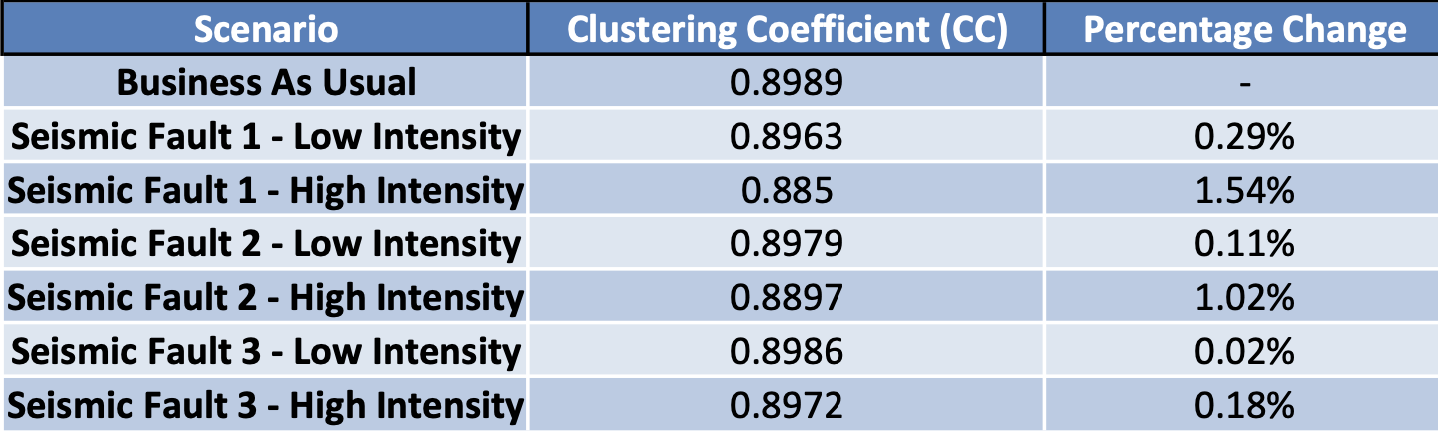
\includegraphics[width=1\textwidth]{images/Table7.png}
\caption{Clustering Coefficient Values and Percentage Change Across Seismic Scenarios}
\label{tab:clustering_coefficient_change}
\end{table}


The clustering coefficient slightly increases in all seismic scenarios, with the highest increase occurring in Seismic Fault 1 - High Intensity (1.54\%). This suggests that after disruptions, some nodes become more clustered as network pathways are restructured to maintain connectivity.

Seismic Fault 2 - High Intensity also shows a notable increase of 1.02\%, confirming that disruptions in this region led to increased local connectivity among surviving nodes. Conversely, Seismic Fault 3 scenarios exhibit the smallest changes (0.02\% to 0.18\%), reinforcing that this region’s network was less affected in terms of local clustering.

\subsection{Interpretation of Results}
The increase in the clustering coefficient across all scenarios suggests that seismic disruptions caused a redistribution of connectivity within local node groups. Instead of an overall loss in connectivity, the transport network adapted by forming denser clusters among remaining functional nodes, maintaining local accessibility despite disruptions.

Seismic Fault 1 had the highest increase in clustering coefficient, indicating that the affected region experienced greater traffic rerouting through local roads, reinforcing connectivity within smaller clusters. Seismic Fault 2 also showed significant clustering effects, but to a lesser extent. Seismic Fault 3 remained largely unchanged, suggesting that this region’s network structure was already optimized for local connectivity.

Despite disruptions, the increase in clustering coefficients indicates that the transport network retains local resilience, ensuring that nearby nodes continue functioning as effective clusters even when certain roads fail.

\subsection{Implications for Seismic Resilience}
The increase in clustering coefficients highlights the importance of local road networks in maintaining accessibility after seismic disruptions. Regions with high clustering coefficient increases, such as Fault 1 and Fault 2, require careful traffic management strategies to prevent congestion in local areas where traffic is redirected.

Since Fault 3 had minimal changes, long-term resilience planning should focus on improving overall connectivity rather than enhancing clustering. Future infrastructure development should consider reinforcing key road segments that link separate clusters, ensuring that local redundancy is maintained while also enhancing regional connectivity.

The clustering coefficient analysis provides insights into how local road networks adapt to disruptions, reinforcing the importance of well-connected node groups in maintaining regional mobility after an earthquake.

\section{Average Degree (CD) Analysis}
\subsection{Average Degree Before Disruption (BAU)}
The average degree (CD) quantifies network connectivity by measuring the average number of links per node. A higher CD value indicates a well-connected network with multiple alternative routes, while a lower CD value suggests a more fragmented network where nodes have fewer connections.

In the Business-As-Usual (BAU) scenario, the average degree is 2.966, indicating that nodes have an average of nearly three connections. This suggests that the transport network in Southern Italy has a relatively well-distributed connectivity structure, ensuring that most nodes maintain access to multiple routes.

\subsection{Changes in Average Degree After Disruption}
Seismic disruptions impact the average degree by reducing the number of functional links, thereby lowering the number of connections per node. The table below summarizes the average degree values before and after disruptions and their percentage change for each scenario.

\begin{table}[H]
\centering
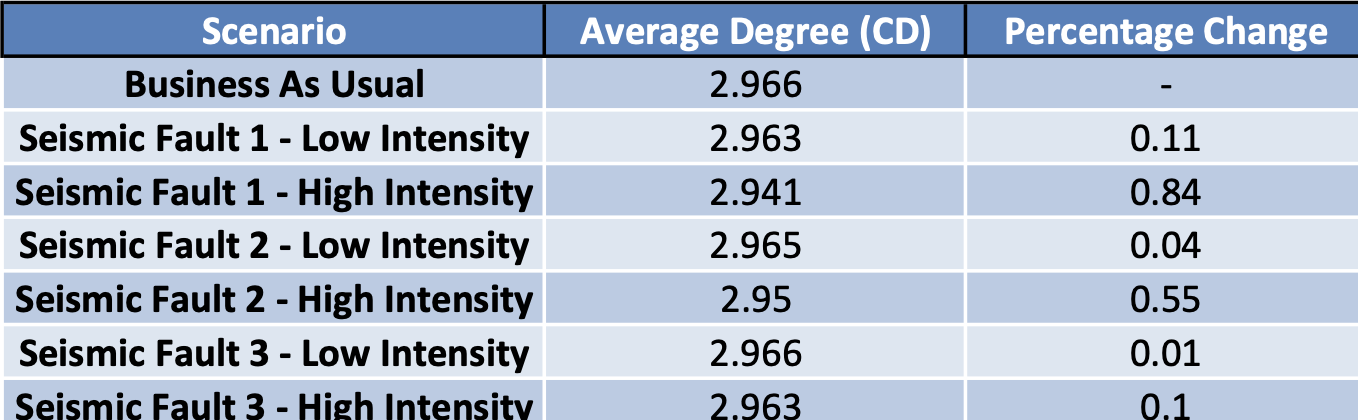
\includegraphics[width=1\textwidth]{images/Table8.png}
\caption{Average Degree Values and Percentage Change Across Seismic Scenarios}
\label{tab:average_degree_change}
\end{table}

The largest drop in average degree occurs in Seismic Fault 1 - High Intensity (0.84\%), indicating that this scenario resulted in the most significant reduction in connectivity. Seismic Fault 2 - High Intensity (0.55\%) also exhibits a noticeable decline, while Seismic Fault 3 scenarios show minimal reductions (0.01\% to 0.10\%), reinforcing that this region was already less connected and, therefore, less affected by disruptions.

\subsection{Interpretation of Results}
Seismic Fault 1 experienced the highest reduction in average degree, reflecting the largest impact on node connectivity. Seismic Fault 2 also showed a moderate decline, suggesting that while this region experienced disruptions, connectivity loss was not as severe as in Fault 1. Seismic Fault 3 remained relatively stable, with only minor changes in connectivity, indicating that its network was already sparse, and disruptions did not significantly alter its structure.

Despite connectivity losses across all scenarios, the percentage changes in average degree remained small, confirming that the transport network still retained some level of redundancy, preventing widespread disconnection.

\subsection{Implications for Seismic Resilience}
Regions with higher reductions in average degree, particularly Fault 1 and Fault 2, require targeted interventions to reinforce network connectivity. Strategies such as adding new links to critical nodes and ensuring that remaining routes can handle detoured traffic are essential for maintaining mobility after an earthquake.

Since Fault 3 had minimal reductions, long-term resilience planning should focus on improving overall connectivity rather than mitigating short-term disruptions. This region’s network needs additional links to increase redundancy, ensuring that future disruptions do not result in complete isolation of affected areas.

The average degree analysis provides valuable insights into how seismic disruptions impact network-wide connectivity, highlighting the importance of reinforcing key road connections to minimize transport system failures after an earthquake.

\section{Redundancy Analysis of the Transport Network Under Seismic Scenarios}
\subsection{Introduction to Redundancy Analysis}
Redundancy in transport networks refers to the system’s ability to maintain connectivity by providing alternative routes when primary roads fail. It is calculated as the ratio of travel time before disruption to travel time after disruption. A redundancy value close to 1 indicates a resilient network with minimal impact on travel time, whereas values approaching 0 signify severe disruptions, leading to complete disconnections.

The graphical representations categorize the zones based on their redundancy levels:

\begin{itemize}
    \item \textbf{Red zones}: These areas have a redundancy value of 0.000, indicating they are completely disconnected after disruption.
    \item \textbf{Blue zones}: These areas have a redundancy value of less than 0.900, meaning they experience increased travel times but remain accessible.
\end{itemize}

This section evaluates how different seismic fault scenarios influence redundancy across the study area. Additionally, OD pair figures illustrate the extent of connectivity loss and increased travel times across different regions, providing a detailed view of affected transport links.

\subsection{ Redundancy Analysis for Seismic Scenarios}
Each seismic fault scenario (low and high intensity) results in varying levels of network disruption. The analysis is based on travel time changes from origin-destination (OD) pairs. 

\subsubsection{Seismic Fault 1}
\begin{itemize}
    \item \textbf{Low-Intensity (8 km radius)}
    \begin{itemize}
        \item Minimal impact on connectivity with other zones compared to other seismic faults.
        \item Only one isolated zone observed, showing a relatively resilient network response.
        \item OD pairs indicate minor travel time increases, but no significant connectivity loss (Figure Y).
    \end{itemize}
    \item \textbf{High-Intensity (15 km radius)}
    \begin{itemize}
        \item A significant expansion of disconnected areas, with a clear increase in red zones.
        \item The number of impacted zones increased as more links failed, leading to widespread network fragmentation.
        \item OD pairs show major disconnections, particularly between Benevento, Avellino, and Napoli, with increased travel times towards Apulia (Figure A).
    \end{itemize}
\end{itemize}

\begin{figure}[H]
\centering
{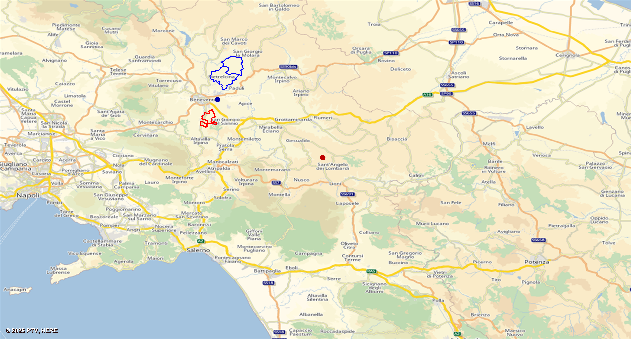
\includegraphics[width=1\textwidth]{images/1.png}}
    \caption{Redundancy map for Seismic Fault 1 – Low Intensity (8 km) - Destination}
\end{figure}

\begin{figure}[H]
\centering
{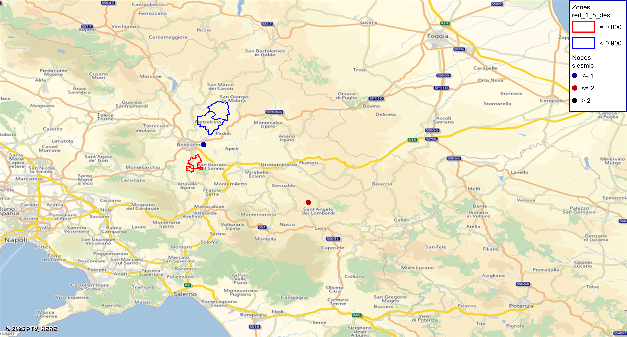
\includegraphics[width=1\textwidth]{images/2.png}}
    \caption{Redundancy map for Seismic Fault 1 – Low Intensity (8 km) - Origin}
\end{figure}


\begin{figure}[H]
\centering
{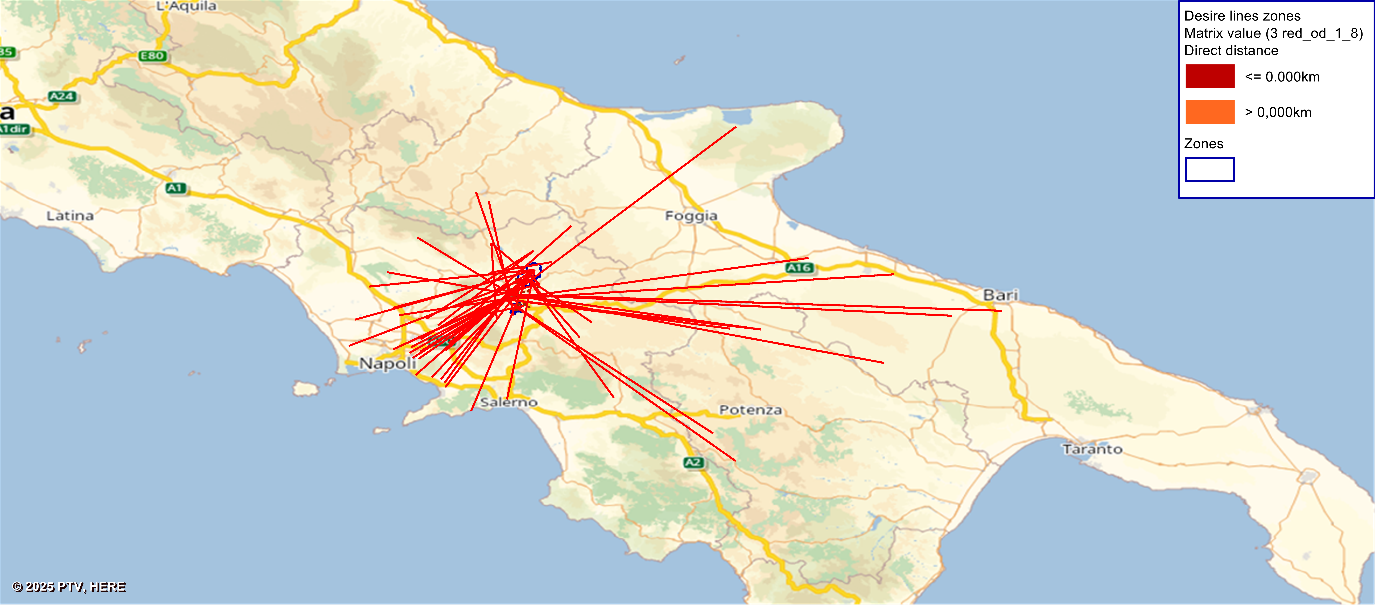
\includegraphics[width=1\textwidth]{images/3.png}}
    \caption{OD Pairs impacted from disruption for Seismic Fault 1}
\end{figure}

\begin{figure}[H]
\centering
{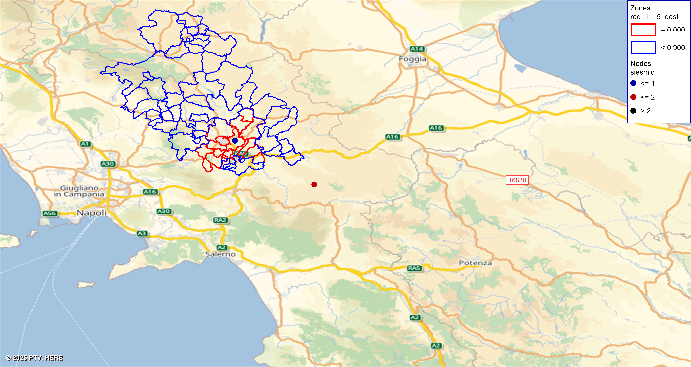
\includegraphics[width=1\textwidth]{images/4.png}}
    \caption{Redundancy map for Seismic Fault 1 – High Intensity (15 km) as Destination}
\end{figure}

\begin{figure}[H]
\centering
{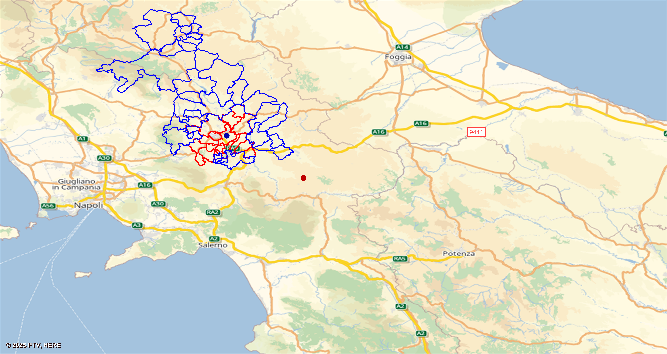
\includegraphics[width=1\textwidth]{images/5.png}}
    \caption{Redundancy map for Seismic Fault 1 – High Intensity (15 km) as Origin}
\end{figure}

\begin{figure}[H]
\centering
{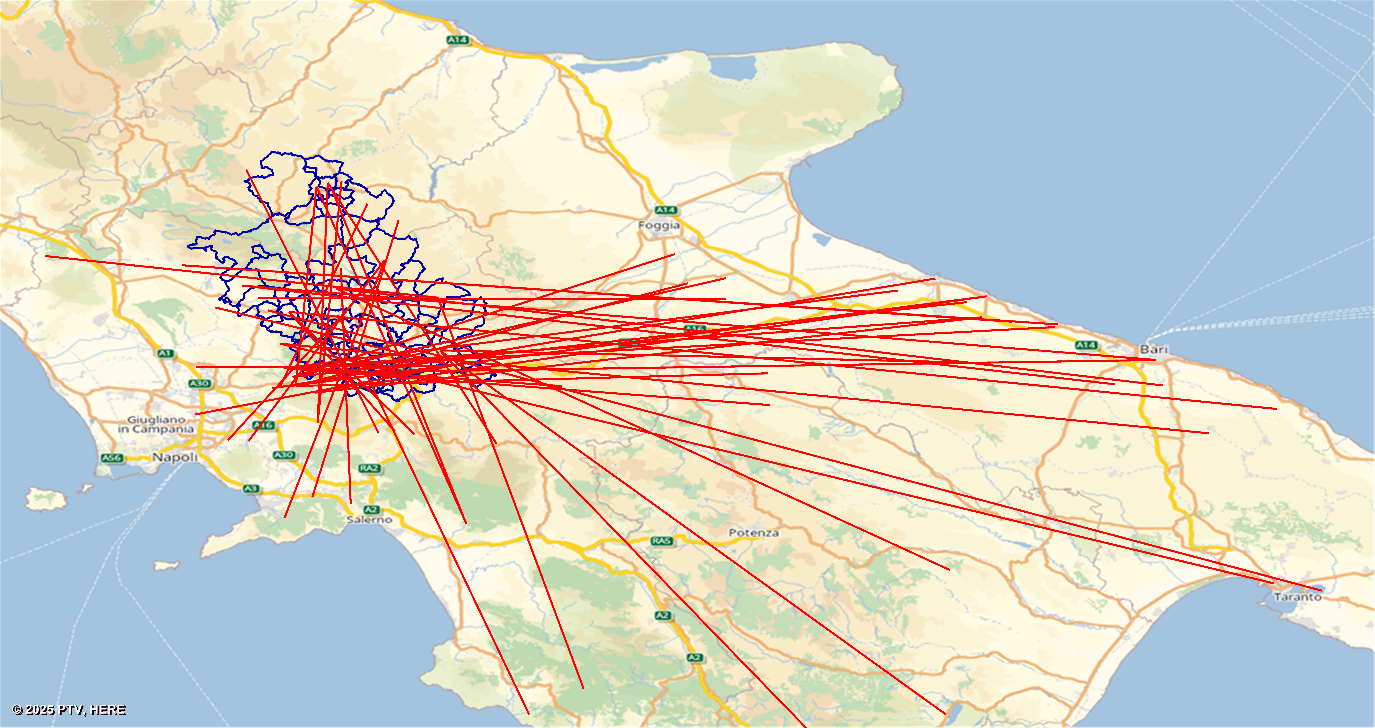
\includegraphics[width=1\textwidth]{images/6.png}}
    \caption{OD Pairs impacted from disruption for Seismic Fault 1(15 km)}
\end{figure}

\subsubsection{Seismic Fault 2}
\begin{itemize}
    \item \textbf{Low-Intensity (8 km radius)}
    \begin{itemize}
        \item No significantly affected zones were observed, indicating a more resilient network structure.
        \item OD pairs reflect a stable connectivity pattern with minor delays.
    \end{itemize}
    \item \textbf{High-Intensity (15 km radius)}
    \begin{itemize}
        \item A significant expansion of disconnected areas, with a clear increase in red zones.
        \item The number of impacted zones increased as more links failed, leading to widespread network fragmentation.
        \item OD pair analysis shows that zones impacted by severe seismic events extended eastward towards Apulia, specifically Bari province, due to limited major roads facilitating east-west connections (Figure D).
    \end{itemize}
\end{itemize}
Under low-intensity scenarios (8 km), the network remained largely intact, showing minimal impacts and no significant isolation.
However, high-intensity scenarios (15 km) had severe consequences, especially around Fault 1 (Benevento) and Fault 2 (Avellino).

Fault 1 scenarios showed the greatest damage, clearly isolating multiple zones—these appear as red zones on the redundancy maps.
Fault 2 had unexpected yet critical effects, extending disruptions significantly eastward towards Bari in Puglia. This impact is due to the limited number of major east-west routes, notably the critical A16 motorway, linking Campania to Puglia.

This eastward expansion of affected zones is due to the lower availability of major roads facilitating east-west connections in the region. When an earthquake occurs, the A16 motorway, which serves as a key east-west connection between Campania and Puglia, becomes severely impacted. Since this is one of the few major corridors linking the western and eastern parts of the region, its disruption leads to extensive accessibility losses. In contrast, Campania, especially Napoli province, has multiple access roads and a more integrated network, which allows it to maintain better connectivity even during disruptions.

\begin{figure}[H]
\centering
{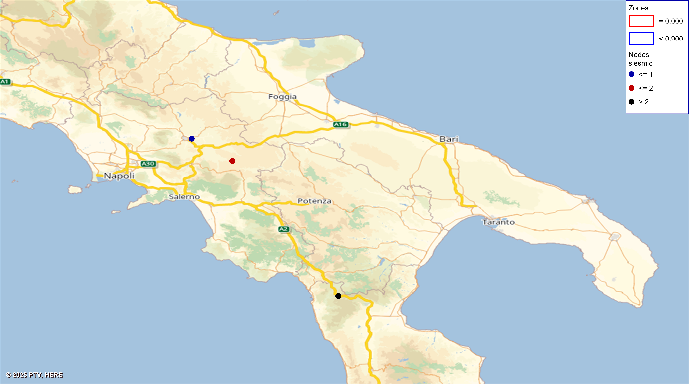
\includegraphics[width=1\textwidth]{images/7.png}}
    \caption{Redundancy map for Seismic Fault 2 – Low Intensity (8 km) as Destination}
\end{figure}

\begin{figure}[H]
\centering
{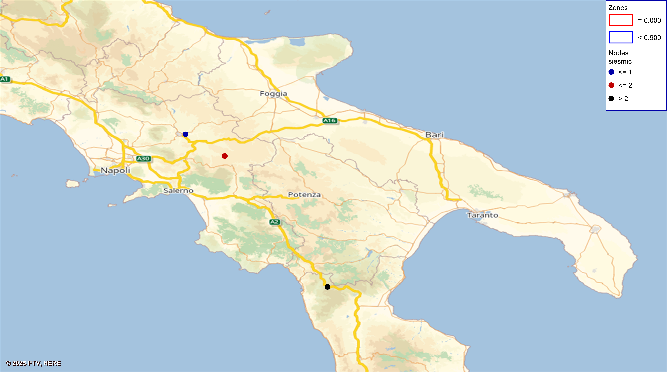
\includegraphics[width=1\textwidth]{images/8.png}}
    \caption{Redundancy map for Seismic Fault 2 – Low Intensity (8 km) as Origin}
\end{figure}

\begin{figure}[H]
\centering
{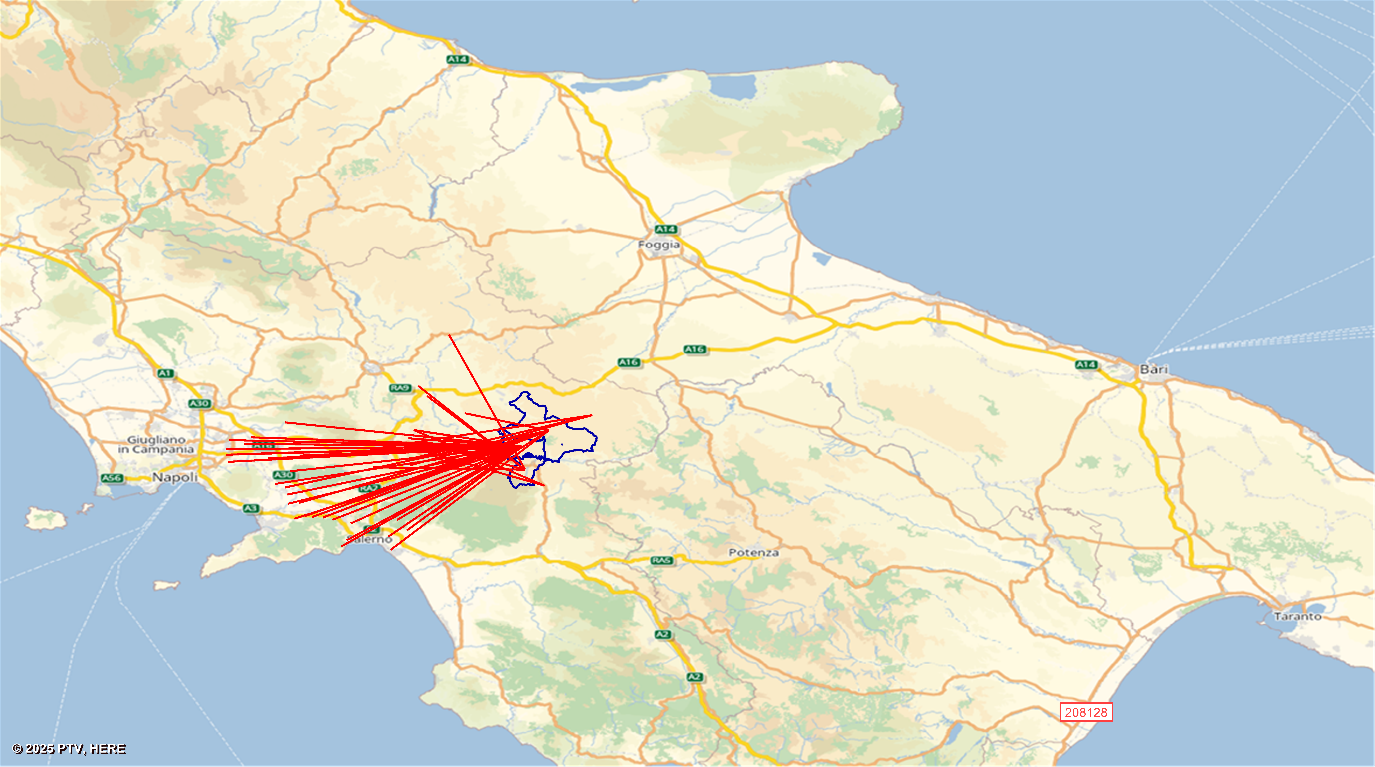
\includegraphics[width=1\textwidth]{images/9.png}}
    \caption{OD Pairs impacted from disruption for Seismic Fault 2 (8 km)}
\end{figure}

\begin{figure}[H]
\centering
{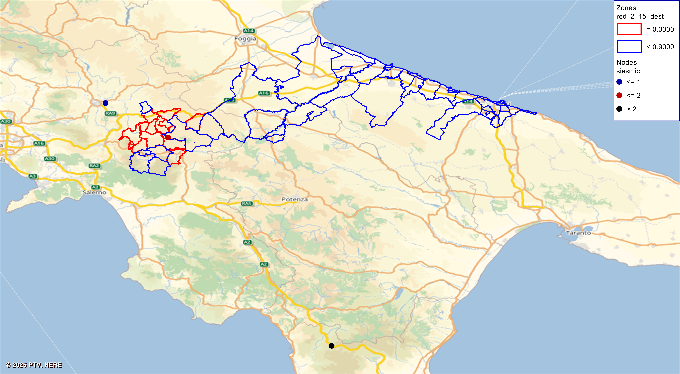
\includegraphics[width=1\textwidth]{images/10.png}}
    \caption{Redundancy map for Seismic Fault 2 – High Intensity (15 km) as Destination}
\end{figure}

\begin{figure}[H]
\centering
{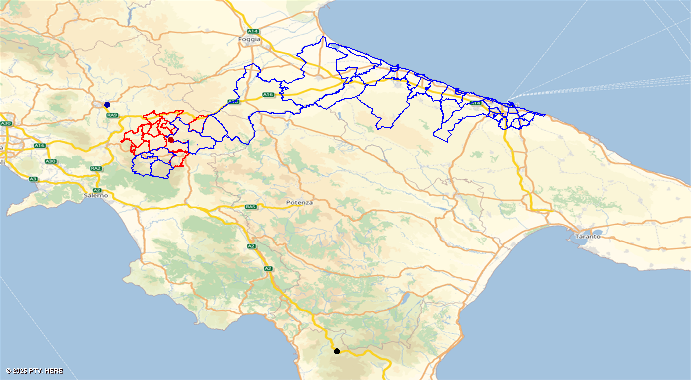
\includegraphics[width=1\textwidth]{images/11.png}}
    \caption{Redundancy map for Seismic Fault 2 – High Intensity (15 km) as Origin}
\end{figure}

\begin{figure}[H]
\centering
{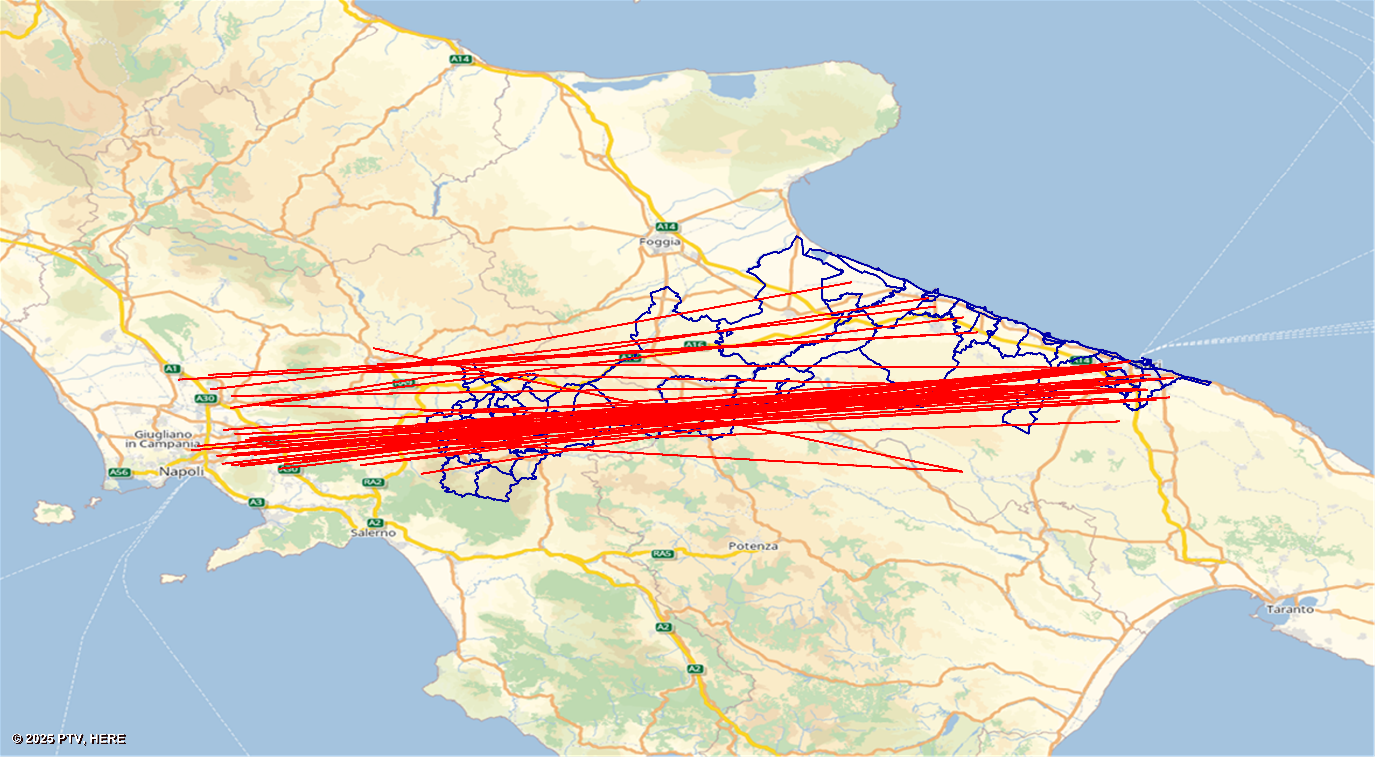
\includegraphics[width=1\textwidth]{images/12.png}}
    \caption{OD Pairs impacted from disruption for Seismic Fault 2 (15 km)}
\end{figure}

\subsubsection{Seismic Fault 3}
\begin{itemize}
    \item \textbf{Low-Intensity (8 km radius)}
    \begin{itemize}
        \item Limited impact on overall redundancy, with only a few zones experiencing travel time increases.
        \item OD pairs confirm that most connections remain intact.
    \end{itemize}
    
    \item \textbf{High-Intensity (15 km radius)}
    \begin{itemize}
        \item A substantial rise in disconnected zones, particularly in Calabria.
        \item The network was vulnerable due to fewer alternative routes and a lower node density.
        \item Although initially the least significant, Fault 3 became a critical scenario in high-intensity disruption, as the destruction of key nodes caused widespread connectivity loss in Calabria, reinforcing its vulnerability.
    \end{itemize}
\end{itemize}

\begin{figure}[H]
\centering
{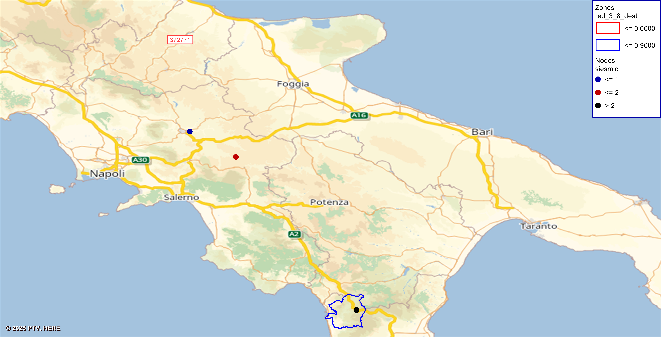
\includegraphics[width=1\textwidth]{images/13.png}}
    \caption{Redundancy map for Seismic Fault 3 – Low Intensity (8 km) as Destination}
\end{figure}

\begin{figure}[H]
\centering
{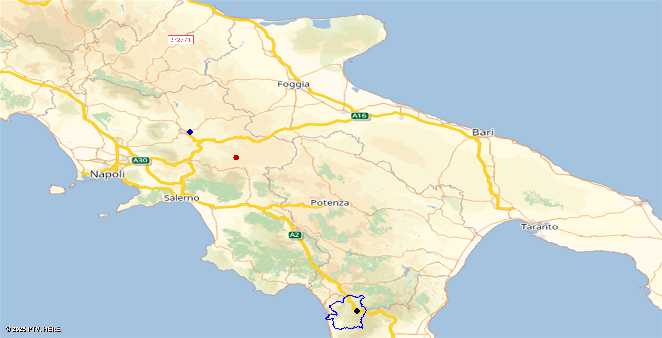
\includegraphics[width=1\textwidth]{images/14.png}}
    \caption{Redundancy map for Seismic Fault 3 – Low Intensity (8 km) as Origin}
\end{figure}

\begin{figure}[H]
\centering
{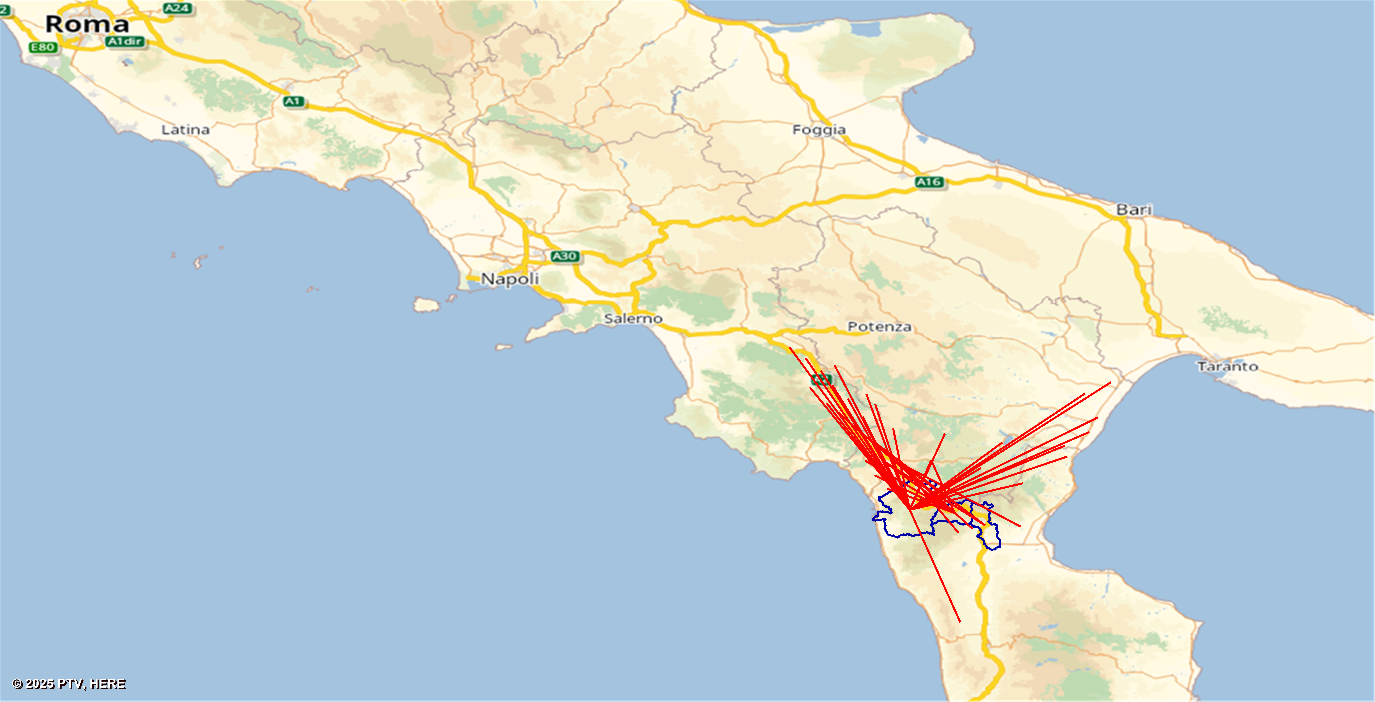
\includegraphics[width=1\textwidth]{images/15.png}}
    \caption{OD Pairs impacted from disruption for Seismic Fault 3 (8 km)}
\end{figure}

\begin{figure}[H]
\centering
{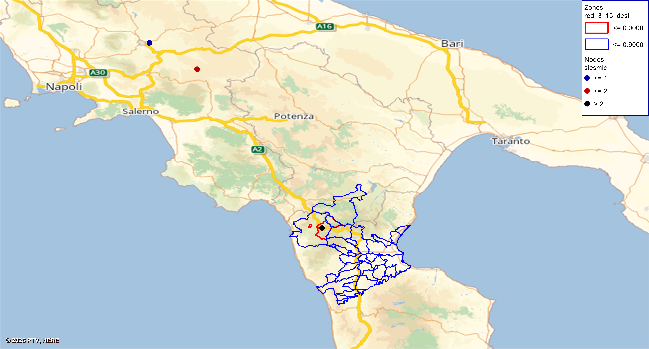
\includegraphics[width=1\textwidth]{images/16.png}}
    \caption{Redundancy map for Seismic Fault 3 – High Intensity (15 km) as Destination}
\end{figure}

\begin{figure}[H]
\centering
{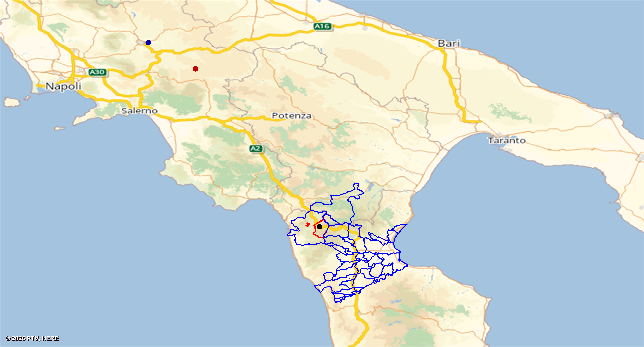
\includegraphics[width=1\textwidth]{images/17.png}}
    \caption{Redundancy map for Seismic Fault 3 – High Intensity (15 km) as Origin}
\end{figure}

\begin{figure}[H]
\centering
{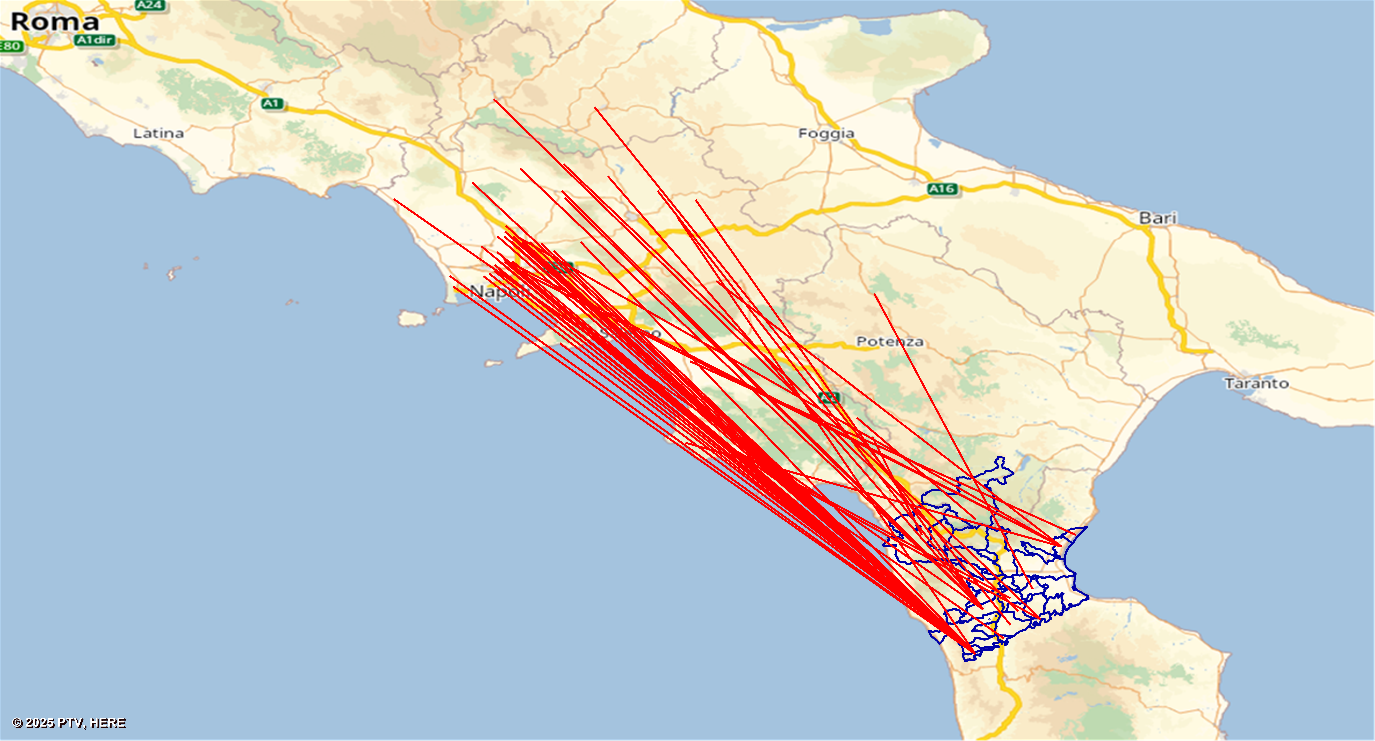
\includegraphics[width=1\textwidth]{images/18.png}}
    \caption{OD Pairs impacted from disruption for Seismic Fault 3 (15 km)}
\end{figure}

\subsection{Findings and Comparative Discussion}
\begin{itemize}
    \item \textbf{Seismic Fault 1} exhibited the most significant impact, particularly in high-intensity scenarios, where multiple red zones emerged, leading to complete disconnections.
    \item \textbf{Seismic Fault 2} displayed moderate effects, with connectivity still preserved in most scenarios, except for the high-intensity case, which caused noticeable disruptions, particularly affecting OD pairs between Campania and Puglia.
    \item \textbf{Seismic Fault 3}, despite being initially the least critical, became the most vulnerable in high-intensity scenarios due to its low node density. The loss of even a few crucial nodes led to widespread disconnections.
    \item \textbf{OD pairs} in high-intensity scenarios consistently showed lower redundancy values, signifying major delays and potential isolation of specific regions.
    \item \textbf{Motorways and major trunk roads} played a key role in maintaining connectivity, but disruptions forced detours onto secondary roads, leading to increased travel times.
\end{itemize}

\subsection{Implications for Seismic Resilience Planning}
\begin{itemize}
    \item \textbf{Highways and major roads} should be reinforced to mitigate cascading failures caused by disruptions.
    \item In \textbf{Benevento and Avellino} (Seismic Fault 2), particularly \textbf{Avellino}, redundancy strategies should be implemented, such as alternative expressways or reinforced detour routes, to minimize isolation risks.
    \item \textbf{Calabria} needs improved redundancy measures, as its low node density makes it highly susceptible to severe connectivity losses in extreme scenarios.
    \item \textbf{Emergency rerouting strategies} should focus on OD pairs with low redundancy values, ensuring minimal travel delays and maintaining regional accessibility.
\end{itemize}

\subsection{ Conclusion}
The redundancy analysis provides a clear picture of network vulnerability under seismic stress. While some regions exhibit greater resilience, others—such as Benevento and Avellino in the Faults 1 and 2 high-intensity scenario—face severe connectivity issues. The OD pair figures confirm the extent of network fragmentation, illustrating critical disconnections and major travel time increases, particularly in east-west transport corridors reliant on the A16 motorway.  By integrating redundancy insights into planning strategies, transport networks can be optimized to withstand future seismic disruptions, ensuring continued mobility and accessibility across Southern Italy.
\chapter{Conclusion}

\section{Summary of Key Findings}
This study assessed the resilience of the transport network in Southern Italy under seismic disruption scenarios, focusing on multiple graph theory indicators to evaluate network performance before and after disruptions. The research identified critical links and nodes, connectivity shifts, and redundancy changes, providing a comprehensive understanding of how different seismic faults impact regional mobility.

\begin{itemize}
    \item \textbf{Betweenness Centrality Analysis} revealed that disruptions shift network importance, concentrating traffic on alternative routes, particularly in Campania and Puglia. The most vulnerable links were motorways and primary roads, emphasizing the importance of maintaining these corridors for network resilience.
    
    \item \textbf{Node Centrality Analysis} showed that intersections near Seismic Fault 1 and Fault 2 played a crucial role in overall connectivity, with high-intensity earthquakes significantly increasing nodal vulnerability.
    
    \item \textbf{Beta Index and Gamma Index} computations highlighted that network connectivity declined significantly after disruptions, especially in high-intensity earthquake scenarios, where many road segments became isolated.
    
    \item \textbf{Clustering Coefficient and Average Degree (CD) Analysis} indicated that local connectivity fragmentation was more pronounced in rural areas, whereas urban areas showed better resilience due to alternative routes.
    
    \item \textbf{Redundancy Analysis} revealed that high-intensity earthquakes caused the complete isolation of several zones, particularly in eastern Campania, where limited alternative routes exacerbated network fragmentation. The A16 motorway was identified as a critical transport corridor, and its disruption led to significant travel time increases and severe accessibility loss, further highlighting the region’s vulnerability to seismic events.
\end{itemize}

The results underscore the necessity of strategic interventions to enhance network robustness against seismic events:

\begin{itemize}
    \item Strengthening critical road corridors, especially motorways and trunk roads, to prevent network fragmentation.
    \item Enhancing redundancy measures in Campania and Calabria is essential, as these regions have fewer alternative routes, making them particularly susceptible to severe disruptions. Strengthening key road links and improving network adaptability can help mitigate the impact of seismic-induced failures and maintain regional mobility.
    \item Enhancing emergency response planning by identifying and prioritizing high-risk links and nodes to minimize congestion and facilitate recovery.
    \item Developing alternative expressways and bypass routes in eastern Campania is crucial to ensuring that seismic disruptions do not severely affect the broader transport network. Strategic investments in new transport corridors and reinforcement of existing infrastructure can enhance regional connectivity and reduce dependency on single critical routes, thereby improving overall network resilience.Utilizing GIS-based and graph-theoretic models for ongoing seismic risk assessment and adaptive infrastructure planning.
    
\end{itemize}

\section{Contributions of the Study}
This research integrates network science and resilience analysis to offer a quantitative evaluation of seismic impacts on transport systems. The study’s main contributions include:

\begin{itemize}
    \item Applying graph theory metrics to evaluate transport network resilience in an interregional context.
    \item Incorporating GIS-based spatial analysis to map and visualize post-disruption connectivity changes.
    \item Providing a structured framework for assessing and improving transport resilience, adaptable to other seismically active regions.
\end{itemize}

\section{Limitations and Future Research}
While this study provides valuable insights, some limitations remain:

\begin{itemize}
    \item The model assumes uniform road disruption probabilities, whereas real-world failures may depend on soil conditions, structural integrity, and traffic loads.
    \item The analysis focuses on road transport, but future studies could incorporate multimodal networks (rail, maritime, air) to assess comprehensive mobility resilience.
    \item Long-term recovery dynamics were not included; future research should explore how disrupted networks gradually regain functionality over time.
    \item Climate-induced disruptions (e.g., floods, landslides) should be considered alongside seismic risks to create a multi-hazard resilience framework.
\end{itemize}

\section{Final Remarks}
This research highlights the critical need for resilient transport infrastructure in Southern Italy, where seismic events pose a significant threat to regional connectivity and economic stability. By combining network analysis, GIS methodologies, and resilience indicators, this study provides actionable recommendations to enhance transport robustness, mitigate disruptions, and support long-term planning efforts. The findings contribute to the broader discourse on transport resilience, emphasizing the role of data-driven decision-making in safeguarding mobility in disaster-prone regions.


\printbibliography
\end{document}
